\documentclass[11pt]{article}
\usepackage[margin=1in]{geometry}
\usepackage{amsmath,amssymb,amsthm}
\usepackage[T1]{fontenc}
\usepackage{lmodern,microtype}
\usepackage{booktabs,array,enumitem}
\usepackage{tikz}
\usetikzlibrary{arrows.meta,positioning,calc}
\usepackage{algorithm,algpseudocode}
\usepackage[section]{placeins}
\setlength{\emergencystretch}{1.5em}
\usepackage[colorlinks=true,linkcolor=blue,citecolor=blue,urlcolor=blue]{hyperref}
\newtheorem{theorem}{Theorem}[section]
\newtheorem{lemma}[theorem]{Lemma}
\newtheorem{corollary}[theorem]{Corollary}
\newtheorem{proposition}[theorem]{Proposition}
\newtheorem{claim}[theorem]{Claim}
\theoremstyle{definition}
\newtheorem{definition}[theorem]{Definition}
\newtheorem{invariant}[theorem]{Invariant}
\theoremstyle{remark}
\newtheorem{remark}[theorem]{Remark}
\newcommand{\sefe}{\textnormal{\textsc{SEFE-2}}}
\newcommand{\Ftwo}{\mathbb F_2}
\newcommand{\rev}{\operatorname{rev}}
\newcommand{\side}{\operatorname{side}}
\newcommand{\gap}{\gamma}
\title{Simultaneous Embedding with Fixed Edges\\When the Common Graph Is a Cactus}
\author{Charlie Cruz}
\date{Draft}
\begin{document}
\maketitle
\begin{abstract}
We give an $O(N^3)$-time algorithm for simultaneous embedding with fixed
edges (\sefe) of two planar graphs whose common graph is a cactus, that is,
every block of the common graph is an edge or a cycle. The common graph may
be disconnected, contain isolated vertices, and have cutvertices of
unbounded degree; the private edges are unrestricted. For positive
instances the algorithm constructs compatible combinatorial embeddings.
Combined with a reduction of Bl\"asius, Karrer and Rutter, the decision
takes the same time when every component of the common graph is a cactus or
$2$-connected.

The proof has two parts. First, a repair theorem characterizes feasibility
by embeddings of the blocks of both inputs that have compatible common edge
orders at every vertex, together with sides of the vertices of each common
cycle's block that depend only on their component of the union minus the
cycle; from these data the block embeddings can be reassembled. Second, we
compile this characterization into a linear-size instance of Synchronized
Planarity augmented by marked cycles, local gap observations and binary
parity constraints. We show how the observations transform under the
operations of Bl\"asius, Fink and Rutter, which we run unchanged up to
subdivided edges, and solve the final instance in linear time.
\end{abstract}

\section{Introduction}\label{sec:intro}

The input to \sefe{} (\emph{simultaneous embedding with fixed edges} of two
graphs) consists of finite simple planar graphs $G_1=(V,E_1)$ and
$G_2=(V,E_2)$ on the same vertex set. The question is whether there are
planar drawings $\Gamma_1$ of $G_1$ and $\Gamma_2$ of $G_2$ such that every
vertex is drawn at the same point in both and every \emph{common} edge
$e\in E_1\cap E_2$ is drawn as the same curve in both. Edges of
$E_1\setminus E_2$ may cross edges of $E_2\setminus E_1$. We call
$H=(V,E_1\cap E_2)$ the \emph{common graph}, its edges \emph{common}, and all
other edges \emph{private}; $G_1$ is the red graph and $G_2$ the blue graph,
and $U=G_1\cup G_2$ is their union.

Simultaneous embeddings were introduced to visualize several related graphs
on one vertex set; see the survey of Bl\"asius, Kobourov and
Rutter~\cite{BKR13}. Gassner, J\"unger, Percan, Schaefer and
Schulz~\cite{GJPSS06} showed that the problem is NP-complete for three input
graphs, and hardness persists when the union has pathwidth at most
five~\cite{DF26}. For two graphs the complexity has remained open. J\"unger
and Schulz~\cite{JS09} showed that a simultaneous embedding exists if and
only if the two inputs have embeddings that induce the same embedding of
$H$: the same cyclic order of common edges around every vertex and the same
relative positions of the components of $H$.

\paragraph{Known tractable cases.}
\sefe{} is polynomial when $H$ is biconnected~\cite{ADFPR12,HJL13}. For
connected $H$, Fulek and T\'oth~\cite{FT22} gave a polynomial algorithm via
atomic embeddability, and Bl\"asius, Fink and Rutter~\cite{BFR21} a
quadratic one via \emph{Synchronized Planarity}. Schaefer~\cite{Sch13}
showed tractability when every component of $H$ is biconnected or has
maximum degree three. Bl\"asius and Rutter~\cite{BR15} solved the case where
the embedding of every component of $H$ is fixed but the relative positions
are free, which includes disjoint cycles. Bl\"asius, Karrer and
Rutter~\cite{BKR18} gave a cubic algorithm for connected inputs in which
the P-nodes and the simultaneous cutvertices (cutvertices of both inputs but
not of their union) have common degree at most three; they also solve
Schaefer's case in cubic time~\cite[Corollary~1(i)]{BKR18}, which covers
cactus common graphs of maximum degree three.
Parameterized algorithms appear in~\cite{FPR25,DF25,DF26}, and Carmesin and
Turner~\cite{CT25} solve a 2-connected version for temporal sequences of
graphs.

These results leave open the combination of a disconnected common graph,
which forces the drawing to decide which face of one component contains
another, with common vertices of high degree whose cyclic order of common
edges is determined by neither input. Bl\"asius, Karrer and Rutter identify
edge orderings at cutvertices as the central difficulty in this
regime~\cite{BKR18}, and Fink~\cite[Section~6.7]{Fin24} asks whether
Synchronized Planarity can be extended to enforce consistent relative
positions when the common graph is disconnected.
Pfretzschner~\cite[Chapter~8]{Pfr22} carried out such an extension when
both inputs are biconnected and have maximum degree four. He augments
Synchronized Planarity with triples consisting of two edges of a
cycle-basis cycle and an attached edge, whose orientations are linked by
parity constraints, shows how the triples transform under the operations,
and obtains a quadratic algorithm~\cite[Theorem~8.16]{Pfr22}; this covers
cactus common graphs, including disconnected ones, when both inputs are
biconnected of maximum degree four. Our local gap observations and their
transport through PropagatePQ follow the same idea. Unbounded degree
requires three further ingredients: new pipes that carry observations, an
inverse for joining two stars that works component by component, and a
permutation of parallel bonds that preserves all gaps.

\paragraph{Our result.}
A \emph{cactus} is a graph in which every block is a single edge or a simple
cycle; equivalently, two cycles share at most one vertex. We allow a
disconnected common cactus with isolated vertices, bridges, and any number
of cutvertices of any degree. $N$ denotes the number of vertices and edges
of the input.

\begin{theorem}\label{thm:main}
\sefe{} can be decided in $O(N^3)$ time for instances whose common graph is
a cactus. For a positive instance, a pair of compatible combinatorial
embeddings, including the relative positions of all components, is
constructed within the same time bound.
\end{theorem}

Time is counted in operations of a word RAM with words of $\Theta(\log N)$
bits. Combined with a reduction of Bl\"asius, Karrer and
Rutter~\cite{BKR18}, the same bound holds when every component of the common
graph is a cactus or $2$-connected (Corollary~\ref{cor:v4i-mixed}).

\subsection{Overview}\label{sec:intro-overview}
The proof has four steps; each section begins by stating its input and
output.

\paragraph{Normalization.}
Using known reductions we make both inputs connected, replace every common
bridge by a common triangle, and split at cutvertices of the union
(Theorem~\ref{thm:v4-normalize}). In the resulting factors $U$ is
biconnected, both colours are connected, and $H$ is a bridgeless cactus plus
isolated vertices.

\paragraph{Repairing block placements.}
For a common cycle $C$ and a component $Z$ of $U-V(C)$, every simultaneous
embedding draws all of $Z$ on one side of $C$, because $Z$ is connected in
$U$ and the curve of $C$ is common. The repair theorem
(Theorem~\ref{thm:v4-repair}) shows that a weak, block-level form of this
condition suffices. It asks only for embeddings of the blocks of both
colours whose common edge orders at every vertex fit together, and in which
the vertices of the block containing $C$ lie on sides of $C$ that depend
only on their component $Z$. The block embeddings are kept, and only the
attachments at cutvertices are rebuilt. The key fact is that at a vertex on
several common cycles the vectors of side bits form a tree with one edge per
cycle, for every choice of the side bits; so the face structure of the
common graph at that vertex is forced.

\paragraph{Compilation.}
Inside a block, the side of a vertex with respect to a common cycle is the
orientation of a triple of directions at one node of an embedding tree: a
rigid reflection, or the gap of a parallel skeleton between the two
directions carrying the cycle (Lemma~\ref{lem:v4-frontier}(c)). We represent all
blocks by their complete families of embedding trees, which have linear
total size (Lemma~\ref{lem:v4-trees}), glue the red and blue trees at every
vertex along common edges, and obtain an instance of Synchronized Planarity
augmented by marked cycles and parity constraints on local gap observations.
It has linear size (Theorem~\ref{thm:v4-compile}).

\paragraph{Local-gap Synchronized Planarity.}
Rigid reflections are native to Synchronized Planarity, whose Q-vertices
are grouped into consistently oriented cells; gap observations are not. We
run the operations of Bl\"asius, Fink and Rutter, unchanged up to
subdivided edges, and show how each
transforms the observations by explicit parity updates
(Theorem~\ref{thm:eng4-main}). The pipe-free instance at the end is solved
in linear time by reading all observations off the embedding trees of its
blocks (Theorem~\ref{thm:eng4-terminal}).

\paragraph{Where the cactus property is used.}
That common rotations and side bits determine the embedding of $H$ does not
need the cactus property: in every connected plane graph the faces are
distinguished by their sides with respect to the cycles, since two faces are
separated by a minimal edge cut of the dual graph, which is a cycle
(compare~\cite[Theorem~8]{BKR18}). The property that
two common cycles share at most one vertex is used in two places. First,
the common cycles through a vertex form a flower, which gives the forced
tree of side vectors in the repair theorem. Second, a parallel skeleton
displays at most one common cycle (Lemma~\ref{lem:v4-display}), so all gap
observations at a P-vertex refer to a single pair of anchors, and for one
anchor pair every assignment of gap bits is realizable. For a common block
that is neither an edge nor a cycle both properties can fail. Arbitrary
families of gap observations at one vertex need not be describable by
parity constraints (Remark~\ref{rem:eng4-anchors}); this limits a direct
extension of our bookkeeping, but does not show that every extension beyond
cacti must fail.

\subsection{Organization}
Section~\ref{sec:v4-prelim} collects preliminaries and the normalization,
Section~\ref{sec:v4-repair} proves the repair theorem,
Section~\ref{sec:v4-lang} defines the target language,
Section~\ref{sec:v4-compile} recalls SPQR and embedding trees and compiles
normalized instances into it, and
Section~\ref{sec:eng4} solves the compiled instances.
Section~\ref{sec:v4i-conclusion} assembles the running time and discusses
open questions. The appendix proves a variant of a normalization lemma
of Bl\"asius and Rutter~\cite{BR15}.

\section{Preliminaries}\label{sec:v4-prelim}

\subsection{Conventions}\label{sec:v4-conv}

All graphs are finite and loopless; multigraphs, whose edges have
identities, are allowed only where this is said. An \emph{instance} of \sefe{} is a pair of simple graphs
$G_1=(V,E_1)$ (red) and $G_2=(V,E_2)$ (blue), with \emph{common graph}
$H=(V,E_1\cap E_2)$ and \emph{union} $U=(V,E_1\cup E_2)$; edges of $H$ are
\emph{common}, the others \emph{private}, and $N=|V|+|E_1|+|E_2|$. A
\emph{cactus} is a graph whose blocks are edges or cycles. We draw on a fixed
oriented sphere $S$; a \emph{SEFE} is a pair of planar drawings of $G_1,G_2$
that coincide on $H$.

\paragraph{Rotation systems.}
A \emph{dart} is an incidence of an edge with one of its ends; $A_v$ is the
set of darts at $v$, $\bar h$ is the dart of the same edge at its other end,
and the dart at $u$ of an edge $uy$ is identified with the traversal
$u\to y$. A \emph{rotation system} $\rho$ gives a cyclic order $\rho_v$ of
$A_v$, the \emph{rotation}, at every vertex $v$, and restricts to subgraphs.
The \emph{successor} of a traversal $u\to y$ is $y\to z$, where the dart of
$yz$ follows that of $yu$ at $y$. The \emph{faces} (\emph{facial walks}) are
the orbits of the successor map together with one (empty) face for every
isolated vertex; this convention is used throughout. Every component $X$ has
$|V(X)|-|E(X)|+f\le2$ ($f$ its number of faces), and $\rho$ is
\emph{planar} if equality holds for every component, i.e.\ genus
$0$~\cite[Chapter~3]{MT01}. Planar rotation systems of connected
graphs are exactly those induced (counter-clockwise) by planar drawings,
which they determine up to orientation-preserving
homeomorphisms~\cite[Chapter~3]{MT01}.

\paragraph{Cyclic orders.}
In a cyclic order $\sigma$, $(x,z)_\sigma$ is the set of elements strictly
between $x$ and $z$ going forward from $x$, and
$\operatorname{or}_\sigma(x,y,z)=0$ if $y\in(x,z)_\sigma$ and $1$ otherwise;
$\operatorname{or}_{\rev\sigma}(x,y,z)=\operatorname{or}_\sigma(z,y,x)
=\operatorname{or}_\sigma(x,y,z)\oplus1$, where $\rev\sigma$ is the reverse
of $\sigma$. For a bijection $\varphi$, $\varphi(\sigma)$ is the image of
$\sigma$; then $(x,z)_{\rev\sigma}=(z,x)_\sigma$ and
$\varphi((x,z)_\sigma)=(\varphi x,\varphi z)_{\varphi\sigma}$. An \emph{interval} is a set of
consecutive elements. Disjoint sets $A,B$ \emph{interleave} if some
$a,a'\in A$, $b,b'\in B$ appear in the cyclic order $a,b,a',b'$; a family is
\emph{noncrossing} if no two members interleave. \emph{Cutting} $\sigma$ at the \emph{corner after} $a$ gives the
linear order from the successor of $a$ to $a$; \emph{inserting} into it
places elements between $a$ and its successor.

\begin{lemma}[intervals]\label{lem:v4-intervals}
Let $\omega$ be a cyclic order of a finite set.
(a) If $\omega$ is the concatenation of nonempty intervals $I_1,\dots,I_m$
and $A,B$ are disjoint, interleave, and meet no common $I_k$, then
$\{k:I_k\cap A\neq\emptyset\}$ and $\{k:I_k\cap B\neq\emptyset\}$
interleave in $(1,\dots,m)$. (b) A noncrossing family of at least two
nonempty sets has a member that is an interval of the restriction of
$\omega$ to the union of the family.
\end{lemma}

\begin{proof}
(a) An interval containing $a,a'$ contains $b$ or $b'$. (b) In the
restriction, a \emph{gap} of $X$ is a maximal set strictly between consecutive
elements of $X$. If no member is an interval, take a nonempty gap $I$ of some
$X$, after $x$, with $|I|$ minimal; a member $X'$ meeting $I$ lies in $I$, and
one of its two nonempty gaps avoids $x$, hence is a smaller gap inside $I$.
\end{proof}

\paragraph{Sides.}
Cycles have length at least two (a \emph{digon}, in a multigraph, has two).
A \emph{directed} cycle $C$ is drawn as a Jordan curve with left side $0$
and right side $1$; $\side(C,Y)$ is the side containing a connected set $Y$
disjoint from $C$. For $u\in V(C)$ the \emph{anchors}
$c_{\mathrm{out}}(C,u)$ and $c_{\mathrm{in}}(C,u)$ are the darts by which
$C$ leaves and enters $u$; the other darts at $u$ are \emph{nonanchor}. For
a cyclic order $\sigma$ of $A_u$ and a nonanchor dart $d$ the \emph{local
gap} is $\gap_\sigma(C,u,d)=\operatorname{or}_{\sigma}(c_{\mathrm{out}}(C,u),
d,c_{\mathrm{in}}(C,u))$, and $\gap_\rho(C,u,d)=\gap_{\rho_u}(C,u,d)$ for a
rotation system $\rho$; so $\gap_\rho(C,u,d)=0$ iff
$d\in(c_{\mathrm{out}}(C,u),c_{\mathrm{in}}(C,u))_{\rho_u}$. In a planar
drawing this sector lies on the left of $C$, so the edge of $d$ leaves $u$
into side $\gap_\rho(C,u,d)$. The \emph{corner side} $\lambda_\rho(C,u,q)$
of a dart $q$ at $u$ is $0$ if $q=c_{\mathrm{out}}(C,u)$, $1$ if
$q=c_{\mathrm{in}}(C,u)$, and $\gap_\rho(C,u,q)$ otherwise; darts $d$
inserted into the corner after $q$ satisfy
$\gap_{\rho'}(C,u,d)=\lambda_\rho(C,u,q)$, since no dart of $C$ separates
them from $q$.

\begin{lemma}[sector]\label{lem:v4-sector}
If $C$ is a directed cycle of a planarly drawn graph with rotation system
$\rho$, $u\in V(C)$, and $Y$ is a connected subgraph with $V(Y)\cap
V(C)=\emptyset$, then $\side(C,Y)=\gap_\rho(C,u,d)$ for the dart $d$ at $u$
of every edge joining $u$ to $Y$, since $Y$ together with these edges,
without their end $u$, is connected and disjoint from $C$.
\end{lemma}

\subsection{Embeddings and common embeddings}\label{sec:v4-emb}

For components $X_a\neq X_b$ of a planarly drawn graph,
$\operatorname{pos}_{X_a}(X_b)$ is the face of $X_a$ containing $X_b$. The
\emph{embedding} of a drawing is its rotation system together with these
\emph{relative positions}. The \emph{containment tree} has as nodes the
components $X_j$ and the components of the complement (\emph{regions}), and
an edge labelled $F$ from $X_j$ to the region meeting $F$ next to $X_j$ for
every face $F$ of $X_j$; it is a tree (Euler characteristic), and
$\operatorname{pos}_{X_a}(X_b)$ labels its first edge towards $X_b$.
Conversely, the edges of $F$ at $X_a$ and $F'$ at $X_b\neq X_a$ meet a common
region iff $F=\operatorname{pos}_{X_a}(X_b)$,
$F'=\operatorname{pos}_{X_b}(X_a)$ and $\operatorname{pos}_{X_c}(X_a)=
\operatorname{pos}_{X_c}(X_b)$ for all $c\neq a,b$, so the positions
determine the tree, which is the undirected auxiliary graph
of~\cite[Sections~4--5]{JS09}; thus our embeddings correspond to their
topological embeddings. Drawings with the same embedding
differ by an orientation-preserving homeomorphism~\cite[Chapter~3]{MT01},
\cite{RS72}, so $\side_{\mathcal E}(C,x)$ is defined for an embedding
$\mathcal E$; and $(G_1,G_2)$ has a SEFE if and only if $G_1,G_2$ have
embeddings inducing the same embedding of $H$~\cite[Theorem~4]{JS09}. For a
cactus this has a local form.

\begin{lemma}[cactus faces]\label{lem:v4-faces}
A planarly drawn connected cactus with $c$ directed cycles has $c+1$ faces;
every face lies on one side of every cycle, and distinct faces have
distinct \emph{side vectors} $(\side(C,F))_C$.
\end{lemma}

\begin{proof}
Add blocks one at a time. An edge keeps the faces and vectors. A cycle $C$
attached at $u$ adds one face: $C-u$ lies in a face $F$, and $F\setminus C$
consists of two faces, on the two sides of $C$, whose vectors differ exactly
in the coordinate of $C$.
\end{proof}

\begin{lemma}[common embeddings]\label{lem:v4-charact}
Let $H$ be a cactus with directed cycles. Embeddings of $G_1$ and $G_2$
induce the same embedding of $H$ if and only if every common dart has the
same rotation at its vertex in both, and $\side_1(C,x)=\side_2(C,x)$ for
every cycle $C$ of $H$ and $x\in V\setminus V(C)$. Such embeddings are
\emph{compatible}; a SEFE exists if and only if compatible embeddings exist.
\end{lemma}

\begin{proof}
Necessity is clear. Conversely, the faces of each component $X$ of $H$ and
their side vectors agree, and for $x$ in a component $X'\neq X$,
$\operatorname{pos}^i_X(X')$ is the face of $X$ with side vector
$(\side_i(C,x))_C$ (Lemma~\ref{lem:v4-faces}).
\end{proof}

\subsection{Block assembly}\label{sec:v4-assembly}

If $W$ is connected and $w\in V(W)$, the blocks $B$ of $W$ at $w$ correspond
to the components $D_B\supseteq B-w$ of $W-w$, and the edges between $w$ and
$D_B$ are those of $B$ at $w$.

\begin{lemma}[assembly]\label{lem:v4-assembly}
Let $W$ be connected and $w\in V(W)$.
\begin{enumerate}[label=(\alph*),nosep]
\item In every planar rotation system of $W$ the dart sets at $w$ of
distinct blocks do not interleave.
\item Let $W=W_1\cup\dots\cup W_m$ with connected $W_k$ that have an edge at
$w$ and pairwise share only $w$, let $\rho_k$ be planar rotation systems of
$W_k$, and let $\sigma$ be a cyclic order of the darts at $w$ restricting to
every $\rho_k(w)$, in which the dart sets of distinct $W_k$ do not
interleave. Then the rotation system with rotation $\sigma$ at $w$ and
$\rho_k$ elsewhere is planar.
\item Given planar rotation systems of all blocks of $W$ and, at every
cutvertex $u$, a cyclic order $\sigma_u$ of its darts restricting to the
rotations of the blocks at $u$ in which the dart sets of distinct blocks do
not interleave, the rotation system of $W$ with these rotations is planar.
\item Let $H$ be a cactus, $G_1,G_2$ connected, $w$ a cutvertex of $U$ with
components $D_1,\dots,D_m$ of $U-w$, and let $\rho^k_1,\rho^k_2$ be
compatible rotation systems of the pair $P_k=(G_1[D_k\cup\{w\}],
G_2[D_k\cup\{w\}])$, whose colours are connected. For each $k$, if $P_k$
has a common dart at $w$, choose one, $q_k$, and cut $\rho^k_1(w)$ and
$\rho^k_2(w)$ at the corner after $q_k$; otherwise cut them anywhere.
Concatenating the cut rotations in the order $k=1,\dots,m$, in both colours,
and keeping all other rotations gives compatible rotation systems of
$(G_1,G_2)$.
\end{enumerate}
\end{lemma}

\begin{proof}
(a) If $a=wy,b,a'=wy',b'$ appear in this order, $a,a'\in B$, $b,b'\in B'$, a
$y$--$y'$ path in $D_B$ closes a cycle avoiding $D_{B'}$ that separates $b$
from $b'$. (b) Induction on $m$. By Lemma~\ref{lem:v4-intervals}(b) the
darts of some $W_m$ form an interval $a_1,\dots,a_p$ of $\sigma$; let $b'$
be the dart before $a_1$. The successor map of $W$ arises from that of
$W'=\bigcup_{k<m}W_k$ and $W_m$, with $w$ doubled, by exchanging the
successors of the traversals entering $w$ along $b'$ and $a_p$, which lie in
different orbits; so $W$ has $f'+f_m-1$ faces and genus $0$. (c) Induction,
splitting at a cutvertex and using (b). (d) Every $x\in D_k$ is joined to $w$ in $G_i$ inside $D_k\cup\{w\}$, and
every cycle of $U$ lies in one $P_k$. Planarity follows from (b), and the
common rotations agree since the common darts of $P_k$ form an interval
starting after $q_k$ in both colours. For a cycle $C$ of $H$ in $P_k$ and
$x\in D_{k'}$, $k'\neq k$, $x$ has the side of $w$ if $w\notin V(C)$, and
otherwise side $\lambda_{\rho^k_i}(C,w,q_k)$, by Lemma~\ref{lem:v4-sector}
applied to the component of $G_i[D_{k'}]$ containing $x$, which is joined to
$w$ by an edge whose dart lies in the corner after $q_k$. This depends only on
common data; apply Lemma~\ref{lem:v4-charact}.
\end{proof}

\subsection{Plane trees}\label{sec:v4-trees}

A \emph{plane tree} is a tree with a rotation system. If it has an edge,
its one face is the \emph{contour}, and the \emph{frontier} is the cyclic
order in which the contour enters the leaves; a single node counts as a leaf
and its frontier is the one-element order of this leaf, as for the embedding
tree of an edge block (Section~\ref{sec:v4-spqr}). The edges \emph{behind} $t\to u$ form the
component of $T-tu$ containing $u$.

\begin{lemma}[plane trees]\label{lem:v4-median}\label{lem:v4-contract}
Let $T$ be a plane tree with an edge and rotation system $\rho$. (a) For an
edge $tu$ the contour is $t\to u$, the traversals of the edges behind
$t\to u$, $u\to t$, and the remaining traversals. (b) If $e_1,\dots,e_k$ are
the edges at $t$ in the order $\rho(t)$, the contour concatenates the
\emph{excursions} along $e_1,\dots,e_k$, each consisting of the traversal
leaving $t$ along $e_l$, those behind it, and the one returning; so the
traversals leaving $t$ appear in the order $\rho(t)$. (c) For a subtree
$T'$ with an edge and the restricted rotations, the contour of $T'$ is the
restriction of that of $T$; reversing all rotations reverses the frontier.
\begin{enumerate}[label=(\alph*),nosep,start=4]
\item (Contraction.) Let $\rho$ be a rotation system of a multigraph $M$ and
$T\subseteq M$ a subtree with an edge, whose inner nodes have all their
darts in $T$ and whose leaves $\ell$ have at most one further dart
$d_\ell$, the edge of which has its other end outside $T$. Contracting $T$
to one vertex whose rotation lists the darts $d_\ell$ in the frontier order
of $T$ preserves the genus of every component. Conversely, replacing a
vertex $w$ by such a tree, with the darts of $w$ attached to its leaves in
frontier order $\rho(w)$, preserves the genus of every component.
\item (Median identity.) Let $a,b,d$ be distinct leaves and $m$ their
\emph{median}, the node on all three paths between them. Then $m$ is an
inner node, the edges $e_a,e_b,e_d$ at $m$ towards $a,b,d$ are distinct,
and $\operatorname{or}_{\mathrm{fr}}(a,d,b)=\operatorname{or}_{\rho(m)}
(e_a,e_d,e_b)$ for the frontier $\mathrm{fr}$.
\end{enumerate}
\end{lemma}

\begin{proof}
(a) After $t\to u$ the contour stays behind $tu$ until it returns; (b)
follows. (c) If the contour leaves $T'$ along an edge, it returns along it
by (a). Reversal replaces the successor $s$ by $rs^{-1}r$, $r$ reversing
traversals. (d) As every $d_\ell$ leaves $T$, each edge of $T$ is the only
edge joining its ends. If $e=tu$ is such an edge, $\rho(t)=(e,a_1,\dots,a_k)$
and $\rho(u)=(e,b_1,\dots,b_l)$, the contracted vertex with rotation
$(b_1,\dots,b_l,a_1,\dots,a_k)$ has the same faces minus the traversals of
$e$ (a single edge becomes an isolated vertex), so genera are kept.
Cutting the edge of each $d_\ell$ into a pendant edge $\ell\ell'$ and
contracting the edges of $T$ one by one keeps the single face of $T$ with
these edges and ends with a star whose rotation is its frontier, the
$\ell'$ in the frontier order of $T$. The converse is the same statement for
the expanded graph. (e) Two leaves behind one edge at $m$ would be joined
avoiding $m$; by (b) $a,b,d$ lie in the excursions of $e_a,e_b,e_d$.
\end{proof}

\subsection{Two noncrossing partitions}\label{sec:v4-partitions}

\begin{lemma}[two noncrossing partitions]\label{lem:v4-partitions}
Let $Y$ be a finite set with a red and a blue partition, every block $X$
carrying a cyclic order $\sigma_X$. Let $M$ be the bipartite multigraph on
the blocks in which each $y\in Y$ is an edge joining its two blocks, with
rotation $\sigma_X$ at red and $\rev\sigma_X$ at blue blocks. This rotation
system is planar if and only if some cyclic order of $Y$ restricts to every
$\sigma_X$ and makes both partitions noncrossing; such an order is computed
in $O(|Y|)$ time.
\end{lemma}

\begin{proof}
Given such an order, place $Y$ on a circle and draw red blocks as stars
inside within the convex hulls of their elements, blue ones likewise
outside. Conversely
(compare~\cite[Lemma~9]{BE18}), draw a component of $M$ planarly with each
edge $y$ subdivided at $m_y$. For every corner $(e,e')$ at a blue vertex,
with red ends $A,A'$, draw an arc from $A$ to $A'$ in the face of the corner
along $e$ and $e'$, leaving $A$ just before $e$ and reaching $A'$ just after
$e'$. These disjoint arcs connect all red vertices; choose a spanning tree of them
by breadth-first search and discard the other arcs. With the red halves of
all edges it forms an embedded tree $\Upsilon$, and the boundary
of a thin neighbourhood of $\Upsilon$ crosses each edge once, near $m_y$, in
the frontier order $\omega$ of the leaves $m_y$. It restricts to the
rotations at red vertices and, from outside, to the reversed rotations at
blue ones; disjoint stars do not interleave. Concatenate over the
components. Combinatorially, the rotation of $\Upsilon$ at a red vertex $A$
is $\rho(A)$ in which the corner between consecutive edges $y,y'$ receives,
in this order, the tree arc of the blue corner ending with $y$ and the tree
arc of the blue corner starting with $y'$ (where these are tree arcs);
$\omega$ is its frontier, computed by face tracing in linear time.
\end{proof}

\subsection{Normalization}\label{sec:v4-normalize}

\begin{definition}\label{def:v4-normalized}
An instance is \emph{normalized} if (N1) $G_1,G_2$ are simple, planar and
connected; (N2) $U$ is biconnected with at least three vertices; (N3) $H$ is
a cactus in which every edge lies on a cycle (isolated vertices allowed).
\end{definition}

\begin{theorem}\label{thm:v4-normalize}
For an instance with planar colours whose common graph is a cactus one
computes in $O(N)$ time normalized instances $I^1,\dots,I^m$ and a set of
one-vertex \emph{trivial factors} such that (a) $\sum_tN(I^t)=O(N)$; (b)
the instance has a SEFE if and only if every $I^t$ has one; (c) from
compatible rotation systems of all $I^t$, compatible embeddings of the
instance, given by rotation systems and containment trees, are computed in
$O(N)$ time.
\end{theorem}

\begin{proof}
Each step preserves simplicity, planarity and the cactus property, and
SEFEs map back by deletion or restriction. \emph{(1)} Treat the components of
$U$ separately; one-vertex components are trivial factors.

\emph{(2) Connecting the colours}, a variant of~\cite[Section~2]{BR15},
whose pendant common edge would be a bridge of $H$. If colour $i$ is
disconnected, let $v_1v_2$ be an edge of $U$ joining two of its components,
private to colour $3-i$. Add vertices $z,t$, the common edges
$v_1z,zt,tv_1$ and the colour-$i$ edge $zv_2$; this merges two components
of $G_i$ and keeps those of $G_{3-i}$. Conversely, by
Lemma~\ref{lem:v4-connect} a SEFE may be assumed to have a face $g$ of
colour $i$ incident with $v_1$ and $v_2$; draw the triangle in a sector at
$v_1$ of the union drawing lying in $g$, and $zv_2$ inside $g$. The edges
$v_1v_2$ of a phase form a spanning tree of $U$ with the components of $G_i$
contracted~\cite[Theorem~1]{BR15}; there are at most $2|V|-2$ steps.

\emph{(3) Bridges.} For every bridge $e=uw$ of $H$ add a vertex $t_e$ and
common edges $ut_e,t_ew$, a block of $H$ as $u,w$ are separated in $H-e$;
in a SEFE nothing crosses $e$, so the triangle can be drawn along it.

\emph{(4) Cutvertices of $U$.} Replace the instance by the pairs $P_k$ of
Lemma~\ref{lem:v4-assembly}(d) at every cutvertex, so that the factors are
induced by the blocks of $U$. No block of $U$ is an edge $xy$: a private
$xy$ has a path in the other colour, a common one lies on a common cycle.
This gives (N1)--(N3).

(a) A step of (2) adds two vertices, three common edges and one private
edge, that is, $9$ to $N$; so (2) adds less than $18|V|$ to $N$, leaving
$|V'|<5|V|$ vertices. Step (3) adds $5$ per bridge, at most $5|V'|$, and
step (4) duplicates only cutvertices,
$\sum_B|V(B)|<2|V''|$; all steps take linear time~\cite{Tar72}. (b) composes
the equivalences.

(c) Undo the splits by Lemma~\ref{lem:v4-assembly}(d), in $O(\deg_U(w))$
time each, obtaining the embeddings of a SEFE of a connected instance.
Deleting $t_e,z,t$ may disconnect the colours; the relative positions are
output as containment trees (Section~\ref{sec:v4-emb}), computed in linear
time since the regions are the classes of faces joined across deleted
edges. Finally, draw the components $U_j$ of $U$ in disjoint disks, in each
colour with the corner after a common dart $d_j$ at a vertex $u_j$ of $U_j$
(any corner if none exists) facing outwards. The complement of the disk of
$U_j$ is connected and avoids $U_j$, so a vertex outside $U_j$ lies on side
$\lambda(C,u_j,d_j)$ of a cycle $C\ni u_j$ of $U_j$, and on the side of $u_j$
otherwise, in both colours (Lemma~\ref{lem:v4-charact}).
\end{proof}

\section{The repair theorem}\label{sec:v4-repair}

Throughout this section $(G_1,G_2)$ is a normalized instance
(Definition~\ref{def:v4-normalized}). Every common edge lies on exactly one
common cycle, the common darts at a vertex $v$ are the darts
$c_{\mathrm{out}}(C,v),c_{\mathrm{in}}(C,v)$ of the common cycles $C$ through
$v$, and $U-v$ is connected for every vertex $v$. Every common cycle $C$
carries one fixed traversal, used in both colours; as a cycle of $G_i$ it
lies in a unique block $B_i(C)$ of $G_i$. Let $\mathcal Z_C$ be the set of
components of $U-V(C)$. Blocks are taken with their colour: a block of $G_1$
and a block of $G_2$ are different objects even if they have the same edges.

\begin{definition}\label{def:v4-datum}
A \emph{block datum} consists of a planar embedding $\mathcal E(B)$ of every
block $B$ of $G_1$ and of $G_2$, and a \emph{side assignment} $s$, a bit
$s(C,Z)$ for every common cycle $C$ and $Z\in\mathcal Z_C$. We write
$s(C,x)=s(C,Z)$ for $x\in Z$, and $s(C,Y)$ for the common value on a
connected subgraph $Y$ of $U-V(C)$.
\end{definition}

\begin{theorem}[repair]\label{thm:v4-repair}
A normalized instance $(G_1,G_2)$ has a SEFE if and only if it has a block
datum such that
\begin{enumerate}[label=(R\arabic*),leftmargin=3em]
\item\label{it:v4-R1} at every vertex $v$ there is a cyclic order $\omega_v$
of the common darts at $v$ that restricts, for every block $B$ of either
colour at $v$, to the order of the common darts of $B$ in $\mathcal E(B)(v)$,
and in which, for $i=1,2$, the partition of the common darts by the blocks
of $G_i$ is noncrossing;
\item\label{it:v4-R2} $\side_{\mathcal E(B_i(C))}(C,x)=s(C,x)$ for every
common cycle $C$, colour $i$ and $x\in V(B_i(C))\setminus V(C)$.
\end{enumerate}
Moreover, from such a datum a SEFE is computed in $O(N^2)$ time; its colour
embeddings restrict to $\mathcal E(B)$ on every block $B$, and every vertex
$x\notin V(C)$ lies on side $s(C,x)$ of every common cycle $C$.
\end{theorem}

The orders $\omega_v$ certify compatibility of the block orders; they need
not be the common rotations of the final embedding.

By Lemma~\ref{lem:v4-partitions}, \ref{it:v4-R1} at $v$ is a planarity
condition on a bipartite map on the blocks at $v$, and $\omega_v$ is computed
in linear time.

\emph{Intuition.} The side assignment fixes on which side of every petal at
$v$ every other petal lies, hence the face tree $T_v$ of the common flower at
$v$ (Figure~\ref{fig:v4-flower}). By~\ref{it:v4-R2} each block's own flower
is a subtree of $T_v$; the old order $\omega_v$ only orders the petals around
each node of $T_v$, the contour of this plane tree is the new common
rotation, and the other darts of each block are attached to it.

\begin{lemma}[necessity]\label{lem:v4-necessary}
Let $(\Gamma_1,\Gamma_2)$ be a SEFE, $C$ a common cycle and $Z\in\mathcal
Z_C$. All vertices of $Z$ lie on one side of $C$, the same in both drawings.
The restrictions of $\Gamma_i$ to the blocks and these sides form a block
datum satisfying~\ref{it:v4-R1} and~\ref{it:v4-R2}, with $\omega_v$ the
common rotation at $v$.
\end{lemma}

\begin{proof}
$C$ is the same closed curve in both drawings. The vertices of $Z$ with the
edges of both colours between them form a connected set avoiding this
curve. The common rotation at $v$ restricts to the order of the common
darts of every block, and the partitions are noncrossing by
Lemma~\ref{lem:v4-assembly}(a); \ref{it:v4-R2} holds since sides do not
change under restriction.
\end{proof}

\subsection{Centres and signature trees}\label{sec:v4-sigtree}

A \emph{centre} is a vertex on at least one common cycle; the common cycles
through a centre $v$ are its \emph{petals}, forming the set $F_v$. They
pairwise share only $v$. For a block $B$ of $G_i$ at $v$ let
\[
J_v(B)=\{C\in F_v: B_i(C)=B\};
\]
these are the petals whose darts at $v$ are darts of $B$, so $B$ has a
common dart at $v$ if and only if $J_v(B)\neq\emptyset$. If $C\in F_v\setminus
J_v(B)$, then $V(B)\cap V(C)=\{v\}$, as distinct blocks share at most one
vertex; moreover $C-v$ lies in the component $D_{B_i(C)}\neq D_B$ of $G_i-v$
(Section~\ref{sec:v4-assembly}). So $D_B$ is connected and disjoint from
$V(C)$, and $s(C,B-v)=s(C,D_B)$ is defined.

Fix a side assignment $s$ and a centre $v$. For a petal $E$ and $b\in\Ftwo$
let $q(E,b)\in\Ftwo^{F_v}$ have $q(E,b)_E=b$ and $q(E,b)_C=s(C,E-v)$ for
$C\neq E$ (the path $E-v$ is connected and disjoint from $V(C)$). The
\emph{signature tree} $T_v(s)$ has the distinct vectors $q(E,b)$ as its
vertices and, for every petal $E$, an edge $E$ joining its \emph{ends}
$q(E,0)\neq q(E,1)$. For a connected subgraph $Y$ of $U-v$ disjoint from
all petals let $q(Y)_C=s(C,Y)$.

\begin{lemma}[signature tree]\label{lem:v4-sigtree}
For every side assignment $s$ and centre $v$, $T_v(s)$ is a tree with
$|F_v|$ edges. For every petal $C$ the two components of $T_v(s)-C$ consist
of the vertices with $C$-coordinate $0$ and $1$, and contain $q(C,0)$ and
$q(C,1)$. For every connected subgraph $Y$ of $U-v$ disjoint from all
petals, $q(Y)$ is a vertex of $T_v(s)$.
\end{lemma}

\begin{proof}
\emph{Forest.} The coordinate $C$ changes along the edge $C$ and along no
other edge, so along a cycle of $T_v(s)$ it would change exactly once.
\emph{Connected.} Call petals $E\neq F$ \emph{adjacent} if a path $P$ in
$U-v$ without inner vertices on petals joins $E-v$ to $F-v$. Cutting a path
of the connected graph $U-v$ at its vertices on petals shows that the
adjacency graph is connected. For adjacent $E,F$ and $C\notin\{E,F\}$ the
set $(E-v)\cup P\cup(F-v)$ is connected and avoids $V(C)$, so
$s(C,E-v)=s(C,F-v)$; hence $q(E,s(E,F-v))=q(F,s(F,E-v))$, and the edges
$E,F$ share an end. So $T_v(s)$ is a tree, the coordinate $C$ is constant on
the components of $T_v(s)-C$, and the ends of $C$ lie in different ones.
\emph{Signatures.} A path in $U-v$ from $Y$ to the petals first meets them
at $w\in E-v$; as the path avoids all other petals before $w$,
$q(Y)_C=s(C,E-v)$ for $C\neq E$, and $q(Y)\in\{q(E,0),q(E,1)\}$.
\end{proof}

\begin{figure}[t]
\centering
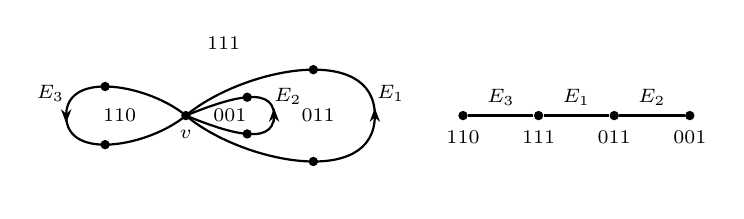
\begin{tikzpicture}[scale=0.8,
  vtx/.style={circle,fill,inner sep=1.2pt},
  lab/.style={font=\scriptsize}]
\begin{scope}
\node[vtx,label={[lab]below:$v$}] (v) at (0,0) {};
\draw[thick] (0,0) to[out=-40,in=-90] node[vtx,pos=0.55]{} (3,0)
  to[out=90,in=40] node[vtx,pos=0.45]{} (0,0);
\draw[thick] (0,0) to[out=-22,in=-90] node[vtx,pos=0.55]{} (1.4,0)
  to[out=90,in=22] node[vtx,pos=0.45]{} (0,0);
\draw[thick] (0,0) to[out=140,in=90] node[vtx,pos=0.55]{} (-1.9,0)
  to[out=-90,in=-140] node[vtx,pos=0.45]{} (0,0);
\draw[-{Stealth[length=5pt]}] (3,-0.12) -- (3,0.12);
\draw[-{Stealth[length=5pt]}] (1.4,-0.1) -- (1.4,0.12);
\draw[-{Stealth[length=5pt]}] (-1.9,0.12) -- (-1.9,-0.12);
\node[lab] at (3.25,0.35) {$E_1$};
\node[lab] at (1.62,0.3) {$E_2$};
\node[lab] at (-2.15,0.35) {$E_3$};
\node[lab] at (0.7,0) {$001$};
\node[lab] at (2.1,0) {$011$};
\node[lab] at (-1.05,0) {$110$};
\node[lab] at (0.6,1.15) {$111$};
\end{scope}
\begin{scope}[xshift=4.4cm]
\node[vtx,label={[lab]below:$110$}] (a) at (0,0) {};
\node[vtx,label={[lab]below:$111$}] (b) at (1.2,0) {};
\node[vtx,label={[lab]below:$011$}] (c) at (2.4,0) {};
\node[vtx,label={[lab]below:$001$}] (d) at (3.6,0) {};
\draw[thick] (a) -- node[lab,above] {$E_3$} (b)
  -- node[lab,above] {$E_1$} (c) -- node[lab,above] {$E_2$} (d);
\end{scope}
\end{tikzpicture}
\caption{A flower with petals $E_1,E_2,E_3$ at $v$, all traversed
counter-clockwise, so that the inside of a petal is its left side $0$
(left), and its signature tree (right). Vectors list the coordinates of
$E_1,E_2,E_3$; for example $q(E_2,0)=001$ because $E_2-v$ lies inside $E_1$
and outside $E_3$. The counter-clockwise order of the six petal darts at $v$
is the contour of the tree (Lemma~\ref{lem:v4-flower}).}
\label{fig:v4-flower}
\end{figure}

\subsection{Flowers inside blocks}\label{sec:v4-flowers}

A \emph{flower} with centre $v$ is a union of directed cycles, its petals,
pairwise sharing exactly $v$. In a planar drawing of a flower $F$ with petal
set $J$, the \emph{face tree} $S(F)$ has the faces as nodes and, for every
petal $P$, an edge $P$ joining the face on side $0$ of $P$ along the edges of
$P$, the end $(P,0)$, to the face on side $1$, the end $(P,1)$.

\begin{lemma}[flowers]\label{lem:v4-flower}
For a planarly drawn flower $F$ with centre $v$, $S(F)$ is well defined and
is a tree; distinct faces have distinct side vectors. The rotation at $v$,
with $c_{\mathrm{out}}(P,v)$ read as the traversal of $P$ from $(P,1)$ to
$(P,0)$ and $c_{\mathrm{in}}(P,v)$ as the reverse, is the contour of $S(F)$
for exactly one rotation system, and the rotation at a node $t$ is then the
restriction of the rotation at $v$ to the darts $c_{\mathrm{out}}(P,v)$ of
the edges $P$ at $t$.
\end{lemma}

\begin{proof}
By Lemma~\ref{lem:v4-faces} $F$ has $|J|+1$ faces with distinct side
vectors. Points near an edge of $P$ on side $b$ of $P$ lie, for $P'\neq P$,
on the side of $P'$ containing $P-v$; so all edges of $P$ have the same face
on side $b$, and the two ends differ. Every face is bounded by an edge of
some petal, so it is an end and touches $v$. A small counter-clockwise
circle around $v$ crosses $c_{\mathrm{out}}(P,v)$ from side $1$ to side $0$
of $P$ and $c_{\mathrm{in}}(P,v)$ the other way; it is a closed walk in
$S(F)$ that visits every node and uses every edge once in each direction, so
$S(F)$ is connected with $|J|+1$ nodes and $|J|$ edges, a tree. Let
$\rho(t)$ map each edge along which the walk enters $t$ to the edge along
which it leaves next. If $\rho(t)$ had several cycles, splitting $t$
accordingly would disconnect the tree, while the walk is a single orbit of
the successor map of the split graph using all edges. So $\rho$ is a
rotation system with the walk as its contour, and it is determined by the
contour. The last statement is Lemma~\ref{lem:v4-median}(b).
\end{proof}

For a block $B$ of $G_i$ at a centre $v$ with $J_v(B)\neq\emptyset$, the
petals in $J_v(B)$ form a flower $F_B\subseteq B$ drawn by $\mathcal E(B)$;
let $S_B=S(F_B)$ with the rotation system of Lemma~\ref{lem:v4-flower}. For
a face $f$ of $F_B$ let $\varphi_B(f)_C$ be the side of $C$ containing $f$ if
$C\in J_v(B)$, and $s(C,B-v)$ otherwise.

\begin{lemma}[block subtrees]\label{lem:v4-subtree}
Assume~\ref{it:v4-R2}. Then $\varphi_B$ is an isomorphism from $S_B$ onto the
subtree $T_B$ of $T_v(s)$ formed by the edges $J_v(B)$ and their ends, mapping
the end $(E,b)$ to $q(E,b)$; every vertex of $T_B$ has $C$-coordinate
$s(C,B-v)$ for $C\notin J_v(B)$.
\end{lemma}

\begin{proof}
Let $f$ be the end $(E,b)$; then $\varphi_B(f)_E=b$. For $C\in J_v(B)$,
$C\neq E$, points near the edges of $E$ lie on the side of $C$ containing
$E-v$, which is $s(C,E-v)$ by~\ref{it:v4-R2}, since $V(E-v)\subseteq
V(B)\setminus V(C)$ and $B=B_i(C)$. For $C\notin J_v(B)$,
$s(C,B-v)=s(C,E-v)$ as $E-v\subseteq B-v$. So $\varphi_B(f)=q(E,b)$. Every
face is an end, so $\varphi_B$ maps nodes to vertices and the edge $E$ to the
edge $E$; it is injective since distinct faces of $F_B$ have distinct side
vectors over $J_v(B)$. An injective map of a tree that sends edges to edges
is an isomorphism onto its image.
\end{proof}

\subsection{Orders at a centre}\label{sec:v4-centre}

\begin{lemma}[private runs]\label{lem:v4-runs}
Let $\mathcal B$ be a set of pairwise disjoint finite sets with cyclic orders
$\theta_B$, and $\emptyset\ne M\subseteq\bigcup\mathcal B$ a set of
\emph{marked} elements. Let $\omega$ be a cyclic
order of $M$ that restricts to $\theta_B|_{M\cap B}$ for every $B$ and in
which the sets $M\cap B$ are noncrossing. Replace every marked $d\in B$ by
$d$ followed by the \emph{run} of unmarked elements that follow $d$ in
$\theta_B$ before the next marked one, and insert every $B$ with $M\cap
B=\emptyset$, cut anywhere, into the corner after the last element of the
run of some marked $d$ (several sets one after another). The result $\omega^+$ restricts to every $\theta_B$, the
sets $B$ are noncrossing in it, and every unmarked element of a set with a
marked element, or inserted after the run of $d$, lies between $d$ and its
successor in $\omega$.
\end{lemma}

\begin{proof}
The runs of $B$ appear in the order of their marked elements, which is
$\theta_B|_{M\cap B}$, so $\omega^+$ restricts to $\theta_B$; inserted sets
are intervals. Suppose sets $B,B'$ with marked elements interleave via
$a,b,a',b'$. Delete the inserted sets; the runs are intervals, and $a,a'$
lie in different runs since an interval containing both would contain $b$
or $b'$. By Lemma~\ref{lem:v4-intervals}(a) the marked heads of the runs of
$a,b,a',b'$ interleave in $\omega$, a contradiction.
\end{proof}

\begin{lemma}[orders at a centre]\label{lem:v4-centre}
Let a block datum satisfy~\ref{it:v4-R1} and~\ref{it:v4-R2}, and let $v$ be a
centre. There are cyclic orders $\omega^1_v,\omega^2_v$ of the darts of $G_1$
and of $G_2$ at $v$ such that
\begin{enumerate}[label=(\roman*),nosep]
\item $\omega^i_v$ restricts to $\mathcal E(B)(v)$ for every block $B$ of
$G_i$ at $v$, and the dart sets of distinct such blocks do not interleave;
\item $\omega^1_v$ and $\omega^2_v$ restrict to the same order of the common
darts;
\item for every block $B$ of $G_i$ at $v$ and $C\in F_v\setminus J_v(B)$,
$\gap_{\omega^i_v}(C,v,d)=s(C,B-v)$ for every dart $d$ of $B$ at $v$.
\end{enumerate}
\end{lemma}

\begin{proof}
Let $T=T_v(s)$ and $\omega_v$ as in~\ref{it:v4-R1}. For a node $t$ of $T$
with edge set $J_t$ let $\rho_t$ be the restriction of $\omega_v$ to the
darts $c_{\mathrm{out}}(E,v)$, $E\in J_t$, read as an order of $J_t$. Let
$\omega'_v$ be the contour of the plane tree $(T,\rho)$, read as an order of
the common darts as in Lemma~\ref{lem:v4-flower}. Let $B$, $B'$ be distinct
blocks of $G_i$ at $v$ with common darts.

(1) \emph{$\omega'_v$ restricts to $\mathcal E(B)(v)$ on the common darts of
$B$.} By Lemma~\ref{lem:v4-flower} and~\ref{it:v4-R1}, the rotation of
$T_B$ at $t$ transported from $S_B$ by Lemma~\ref{lem:v4-subtree} is the
restriction of $\omega_v$, hence of $\rho_t$. So $T_B$ with the restricted
rotations is $S_B$, and by Lemma~\ref{lem:v4-median}(c) the restriction of
$\omega'_v$ is the contour of $S_B$, which is the order of the petal darts
in $\mathcal E(B)(v)$ (Lemma~\ref{lem:v4-flower}).

(2) \emph{The common darts of $B$ and $B'$ do not interleave in $\omega'_v$.}
The subtrees $T_B,T_{B'}$ are edge-disjoint, so they share at most one node.
If they share none, let $e$ be the edge by which the path from $T_B$ to
$T_{B'}$ leaves $T_B$; by Lemma~\ref{lem:v4-median}(a) the traversals behind
$e$ form an interval containing the darts of $B'$ and none of $B$. If they
share $t$, every edge of $T_B$ is at $t$ or behind an edge of $T_B$ at $t$,
and no edge of $T_{B'}$ is behind one; so the darts of $B$ and $B'$ lie in
the excursions (Lemma~\ref{lem:v4-median}(b)) along $J_v(B)\cap J_t$ and
$J_v(B')\cap J_t$, which do not interleave in $\rho_t$ by~\ref{it:v4-R1}, and
Lemma~\ref{lem:v4-intervals}(a) applies.

(3) \emph{Let $C\in F_v$ and let $T^C_b$ be the component of $T-C$ with
$C$-coordinate $b$. For a common dart $q$ whose traversal ends in $T^C_b$,
$\lambda_{\omega'_v}(C,v,q)=b$.} By Lemma~\ref{lem:v4-median}(a) for the
traversal $c_{\mathrm{out}}(C,v)$, from $q(C,1)$ to $q(C,0)$, the open
interval $(c_{\mathrm{out}}(C,v),c_{\mathrm{in}}(C,v))_{\omega'_v}$ consists
of the traversals of the edges of $T^C_0$; a traversal of an edge of $T^C_b$
ends in $T^C_b$, $c_{\mathrm{out}}(C,v)$ ends in $T^C_0$ and
$c_{\mathrm{in}}(C,v)$ in $T^C_1$.

\emph{Completion.} Fix $i$. A block $Y$ of $G_i$ at $v$ without common darts
has $Y-v$ disjoint from all petals, so $q_Y=q(Y-v)$ is a vertex of $T$
(Lemma~\ref{lem:v4-sigtree}); choose a common dart $d_Y$ whose traversal
ends at $q_Y$. Apply Lemma~\ref{lem:v4-runs} to $\omega'_v$, the rotations
$\mathcal E(B)(v)$ of the blocks of $G_i$ at $v$ and the common darts as
marked elements (there are some, as $v$ is a centre, and each is a dart of a
block of $G_i$ at $v$), inserting every such $Y$ after the run of $d_Y$; let
$\omega^i_v$ be the result. Its hypotheses hold by (1) and (2), which gives
(i), and (ii) holds by construction. For (iii) let $b=s(C,B-v)$. If $B$ has
common darts, $T_B$ avoids the edge $C$ and its vertices have
$C$-coordinate $b$ (Lemma~\ref{lem:v4-subtree}), so $T_B\subseteq T^C_b$; a
common dart $d$ of $B$ is not a dart of $C$, so
$\gap_{\omega^i_v}(C,v,d)=\lambda_{\omega'_v}(C,v,d)=b$ by (3), and every
private dart of $B$ lies in the corner after a common dart of $B$
(Lemma~\ref{lem:v4-runs}). If $B=Y$ has none, its darts lie in the corner
after $d_Y$, whose traversal ends at $q_Y\in T^C_b$, and (3) applies.
\end{proof}

\subsection{Proof of the repair theorem}\label{sec:v4-global}

\begin{proof}[Proof of Theorem~\ref{thm:v4-repair}]
Necessity is Lemma~\ref{lem:v4-necessary}. Let a block datum
satisfy~\ref{it:v4-R1} and~\ref{it:v4-R2}. For $i=1,2$ let $\mathcal E'_i$ be
the rotation system of $G_i$ with rotation $\omega^i_v$
(Lemma~\ref{lem:v4-centre}) at every centre $v$, the rotation of
$\mathcal E(B)$ at every other vertex that lies in one block $B$, and at every
other cutvertex the concatenation of the rotations of its blocks, each cut
anywhere. By Lemma~\ref{lem:v4-centre}(i) and
Lemma~\ref{lem:v4-assembly}(c), $\mathcal E'_i$ is planar and restricts to
$\mathcal E(B)$ on every block $B$ of $G_i$; it is an embedding since $G_i$
is connected. Every common dart is at a centre, so by
Lemma~\ref{lem:v4-centre}(ii) the common rotations agree.

\emph{Sides.} Let $C$ be a common cycle, $x\notin V(C)$ and $B=B_i(C)$. We
show $\side_{\mathcal E'_i}(C,x)=s(C,x)$. If $x\in V(B)$ this
is~\ref{it:v4-R2}, as $\mathcal E'_i$ restricts to $\mathcal E(B)$.
Otherwise the path in the block-cut tree of $G_i$ from $B$ to $x$ leaves $B$
at a cutvertex $w\in V(B)$, and $x$ lies in a component $D$ of $G_i-w$ with
$V(D)\cap V(B)=\emptyset$; $D=D_{B'}$ for a block $B'\neq B$ at $w$.
If $w\notin V(C)$, $D\cup\{w\}$ is connected and avoids $V(C)$, so $x$ has
the side of $w$, which is $s(C,w)=s(C,x)$ by the first case. If $w\in V(C)$,
then $w$ is a centre, $C\in F_w\setminus J_w(B')$, and by
Lemma~\ref{lem:v4-centre}(iii) and Lemma~\ref{lem:v4-sector}
$\side_{\mathcal E'_i}(C,D)=s(C,B'-w)=s(C,x)$, since $D$ is connected in
$U-V(C)$ and contains $B'-w$ and $x$. By Lemma~\ref{lem:v4-charact},
$\mathcal E'_1,\mathcal E'_2$ are the embeddings of a SEFE with the stated
properties.

\emph{Time.} Labelling the components of all $U-V(C)$ takes $O(N^2)$ time.
At a centre $v$ with $k_v=|F_v|\le\delta_v=\deg_{G_1}(v)+\deg_{G_2}(v)$,
$\omega_v$ takes $O(\delta_v)$ time (Lemma~\ref{lem:v4-partitions}),
$T_v(s)$ takes $O(k_v^2)$ by radix sort of the vectors $q(E,b)$, locating the
$q_Y$ takes $O(k_v\delta_v)$ with a binary trie, and the contour and runs
take $O(\delta_v)$; in all $O(N^2)$, and the assembly is linear.
\end{proof}

\subsection{Lobes}\label{sec:v4-lobes}

\begin{lemma}[counting]\label{lem:v4-count}
Let $W$ be a biconnected loopless multigraph with at least three vertices
and $\mathcal C$ a set of cycles of $W$ whose union is a cactus. Then
$\sum_{C\in\mathcal C}\operatorname{cc}(W-V(C))\le2|E(W)|$, where
$\operatorname{cc}$ counts components.
\end{lemma}

\begin{proof}
Each $C\in\mathcal C$ is a block of the cactus $\bigcup\mathcal C$. Root
every component of its block-cut tree at a block, and let $r_C$ be the
parent cutvertex of $C$, or any vertex of $C$ if $C$ is a root. The sets
$V(C)\setminus\{r_C\}$ are pairwise disjoint: a vertex $u$ on several members
is a cutvertex of the cactus, and all blocks at $u$ except its parent are
children of $u$. Let $Y$ be a component of $W-V(C)$. If $Y$ had at most one
neighbour on $C$, this neighbour would be a cutvertex of $W$, or $W$ would be
disconnected; so we may charge $Y$ to an edge $yz$ with $y\in Y$ and $z\in
V(C)\setminus\{r_C\}$. Through its end $z$ an edge is charged at most once,
since $z$ determines $C$ and $y$ determines $Y$. So every edge is charged at
most twice.
\end{proof}

Hence $\sum_C|\mathcal Z_C|\le2|E(U)|$ ($W=U$), and, applied to the
blocks of $G_1,G_2$ containing common cycles, the graphs $B_i(C)-V(C)$ have
at most $2(|E_1|+|E_2|)$ components in all.

\section{The target language}\label{sec:v4-lang}

We define the instances that the compiler (Section~\ref{sec:v4-compile})
produces and the engine (Section~\ref{sec:eng4}) decides. Graphs here are
loopless multigraphs; darts, $A_v$, $\bar h$, rotation systems, faces and
planarity, cyclic orders with $\rev$ and images $\varphi(\sigma)$, sides,
anchors and local gaps are as in Section~\ref{sec:v4-conv}.

Informally, the underlying instance is one of Synchronized
Planarity~\cite{BFR21}: P-vertices have free rotations, pipes synchronize
the rotations of pairs of P-vertices, and Q-vertices have fixed rotations up
to reversal; here Q-vertices are grouped into Q-cells that reverse together
according to one flip variable. Some cycles are marked, and distinct marked
cycles share only Q-vertices, so a P-vertex has at most one distinguished
anchor pair. An observer is a Boolean variable that records which of the two
gaps between these anchors contains a specified dart. Binary parity rows
relate observations, Q-cell flips and free Boolean variables.

\begin{definition}[instance]\label{def:v4-instance}
An \emph{instance} is a tuple
$\mathcal I=(G,Q,\psi,f,\mathcal P,\mathcal M,X,\operatorname{obs},R)$ with
the following components.
\begin{enumerate}[label=(\arabic*),nosep]
\item $G$ is a loopless multigraph and $Q\subseteq V(G)$. Every $q\in Q$ (a \emph{Q-vertex}) has a
  \emph{reference rotation} $\psi(q)$, a rotation of $q$, and a \emph{flip
  variable} $f(q)\in X$. The map $f:Q\to X$ need not be injective; its
  nonempty fibres are the \emph{Q-cells}. The vertices not in $Q$ are
  \emph{P-vertices}.
\item $\mathcal P$ is a set of \emph{pipes} $(u,v,\varphi)$: $u\ne v$ are
  P-vertices of equal degree and $\varphi:A_u\to A_v$ is a bijection;
  $(u,v,\varphi)$ and $(v,u,\varphi^{-1})$ are identified, and every
  P-vertex lies in at most one pipe.
\item $\mathcal M$ is a set of \emph{marked cycles} satisfying the
  \emph{marked-cycle invariant}:
  \begin{enumerate}[label=(M\arabic*),nosep]
  \item\label{it:v4-M1} each is a directed simple cycle of $G$ of length at
    least two;
  \item\label{it:v4-M2} they are pairwise edge-disjoint;
  \item\label{it:v4-M3} two distinct marked cycles share only Q-vertices;
  \item\label{it:v4-M4} every pipe $(u,v,\varphi)$ is \emph{off} (neither
    $u$ nor $v$ lies on a marked cycle) or \emph{aligned}: $u\in C$, $v\in C'$
    for marked cycles $C,C'$, and
    $\varphi(\{c_{\mathrm{out}}(C,u),c_{\mathrm{in}}(C,u)\})=
    \{c_{\mathrm{out}}(C',v),c_{\mathrm{in}}(C',v)\}$.
  \end{enumerate}
\item $X$ is a finite set of Boolean variables, and $\operatorname{obs}$ is a
  partial map on $X$ whose values are \emph{observable triples} $(C,v,d)$:
  $C\in\mathcal M$, $v$ a P-vertex of $C$, and $d$ a nonanchor dart at $v$. A
  variable in the domain of $\operatorname{obs}$ is an \emph{observer} of its
  triple.
\item $R$ is a set of \emph{rows} $x\oplus y=c$ with $x,y\in X$ and
  $c\in\Ftwo$. The case $x=y$ is allowed: the row $x\oplus x=0$ always holds
  and the row $x\oplus x=1$ never does.
\end{enumerate}
The \emph{size} $|\mathcal I|$ is the number of vertices and edges of $G$
plus the total length of the bijections of the pipes, of the reference
rotations and of the marked cycles, plus $|X|+|R|$.
\end{definition}

By~\ref{it:v4-M3} a P-vertex $v$ lies on at most one marked cycle $C(v)$.
Members of one Q-cell may lie in
different components of $G$.

\begin{definition}[witness]\label{def:v4-witness}
A \emph{witness} of $\mathcal I$ is a pair $(\rho,\alpha)$ of a planar
rotation system $\rho$ of $G$ and an assignment $\alpha:X\to\Ftwo$ such that
\begin{enumerate}[label=(W\arabic*),nosep]
\item\label{it:v4-W1} $\rho_v=\rev\varphi(\rho_u)$ for every pipe
  $(u,v,\varphi)$;
\item\label{it:v4-W2} for every $q\in Q$ with $\deg q\ge3$,
  $\rho_q=\psi(q)$ if $\alpha(f(q))=0$ and $\rho_q=\rev\psi(q)$ if
  $\alpha(f(q))=1$ (a Q-vertex of degree at most two is unconstrained);
\item\label{it:v4-W3} $\alpha(x)=\gap_\rho(\operatorname{obs}(x))$ for every
  observer $x$;
\item\label{it:v4-W4} every row holds.
\end{enumerate}
The \emph{feasible set} is $F(\mathcal I)=\{\alpha:\exists\rho\
(\rho,\alpha)\text{ is a witness}\}$, and $\mathcal I$ is \emph{feasible} if
$F(\mathcal I)\ne\emptyset$.
\end{definition}

No condition refers to relative positions of components.
Condition~\ref{it:v4-W1} does not depend on the orientation of the pipe.

\begin{definition}[contract]\label{def:v4-contract}
A \emph{step} maps an instance $\mathcal I$ to a rejection or to an instance
$\mathcal I'$ with $X\subseteq X'$. It \emph{satisfies the contract} if it
rejects only when $F(\mathcal I)=\emptyset$, and otherwise, for every
$\alpha:X\to\Ftwo$, from every witness $(\rho,\alpha)$ of $\mathcal I$ one
constructs a witness $(\rho',\alpha')$ of $\mathcal I'$ with
$\alpha'|_X=\alpha$, and from every witness $(\rho',\alpha')$ of
$\mathcal I'$ one constructs $\rho$ such that $(\rho,\alpha'|_X)$ is a
witness of $\mathcal I$.
\end{definition}

Then $F(\mathcal I)=\{\alpha'|_X:\alpha'\in F(\mathcal I')\}$ if the step
does not reject, and steps satisfying the contract compose.

\paragraph{Relocation and canonical observers.}
\emph{Relocating} an observer $x$ to $y\oplus c$, for a variable $y$ and
$c\in\Ftwo$, removes $x$ from the domain of $\operatorname{obs}$ and adds the
row $x\oplus y=c$; $x$ stays a variable. An instance is \emph{canonical} if
no observable triple has two observers. In a canonical instance
$\langle t\rangle$ denotes the observer of the observable triple $t$ if there
is one, and otherwise a fresh variable $x$, added to $X$ with
$\operatorname{obs}(x)=t$; all constructions create observers only in this
way. An instance is made
canonical by keeping one observer $x_t$ of each triple $t$ and relocating
every other observer of $t$ to $x_t\oplus0$; this satisfies the contract,
because the relocated variables keep their values in every witness. When a step
keeps all old rows, checking a new witness amounts to checking
planarity, \ref{it:v4-W1}--\ref{it:v4-W3} and the new rows.

\begin{lemma}[gap facts]\label{lem:v4-gaps}
Let $v$ lie on a directed simple cycle $C$ of a loopless multigraph $W$, and
let $d$ be a nonanchor dart at $v$.
\begin{enumerate}[label=(\alph*),nosep]
\item $\gap_{\rev\sigma}(C,v,d)=1\oplus\gap_\sigma(C,v,d)$ for every rotation
  $\sigma$ of $v$.
\item \emph{(Transfer.)} Let $u\in V(C)$ and $v'\in V(C')$ for directed
  simple cycles $C,C'$, let $\varphi:A_u\to A_{v'}$ be a bijection with
  $\varphi(\{c_{\mathrm{out}}(C,u),c_{\mathrm{in}}(C,u)\})=
  \{c_{\mathrm{out}}(C',v'),c_{\mathrm{in}}(C',v')\}$ (for instance an aligned
  pipe), and let
  $\varepsilon(\varphi)=0$ if $\varphi$ exchanges the anchor types, that is,
  $\varphi(c_{\mathrm{out}}(C,u))=c_{\mathrm{in}}(C',v')$, and
  $\varepsilon(\varphi)=1$ otherwise. If $\rho_{v'}=\rev\varphi(\rho_u)$, then
  $\varphi(e)$ is nonanchor and
  $\gap_\rho(C,u,e)\oplus\gap_\rho(C',v',\varphi(e))=\varepsilon(\varphi)$ for
  every nonanchor dart $e$ at $u$.
\end{enumerate}
\end{lemma}

\begin{proof}
(a) is the identity for $\operatorname{or}_{\rev\sigma}$
(Section~\ref{sec:v4-conv}). (b) Write $o=c_{\mathrm{out}}(C,u)$ and $i=c_{\mathrm{in}}(C,u)$. Since
$\varphi$ maps $\{o,i\}$ onto the anchors at $v'$, $\varphi(e)$ is
nonanchor. Moreover
$e\in(o,i)_{\rho_u}$ if and only if $\varphi(e)\in(\varphi o,\varphi
i)_{\varphi\rho_u}=(\varphi o,\varphi i)_{\rev\rho_{v'}}=(\varphi i,\varphi
o)_{\rho_{v'}}$. If $\varphi$ exchanges the anchor types, the last interval
is $(c_{\mathrm{out}}(C',v'),c_{\mathrm{in}}(C',v'))_{\rho_{v'}}$ and the two
gaps are equal; otherwise it is $(c_{\mathrm{in}}(C',v'),
c_{\mathrm{out}}(C',v'))_{\rho_{v'}}$ and the gaps differ.
\end{proof}

\section{Compilation}\label{sec:v4-compile}

The input of this section is a normalized instance $(G_1,G_2)$
(Definition~\ref{def:v4-normalized}) in which every common cycle carries a
fixed traversal, used in both colours. The output is an instance $\mathcal I$
(Definition~\ref{def:v4-instance}) of size $O(N)$, computed in $O(N^2)$ time,
that is feasible if and only if $(G_1,G_2)$ has a SEFE, with witnesses
translated both ways (Theorem~\ref{thm:v4-compile}). We represent every block
by its embedding trees at all its vertices and join, at every vertex, the red
and the blue leaf of each common dart. Condition~\ref{it:v4-R1} of
Theorem~\ref{thm:v4-repair} becomes planarity, and~\ref{it:v4-R2} a parity
condition on the orientation at the median of the two leaves of $C$ and a
leaf leading off $C$.

\subsection{SPQR trees and embedding trees}\label{sec:v4-spqr}

This subsection collects the facts on SPQR trees used by the compiler and
the engine. Let $B$ be a biconnected loopless planar multigraph that is
neither an edge nor a cycle (a digon is a cycle), and $\mathcal T_B$ its SPQR tree~\cite{DT96},
computed in linear time~\cite{GM01,HT73}. We use the standard
facts~\cite{DT96}, \cite[Section~2.5]{BR16}:
\begin{enumerate}[label=(T\arabic*),nosep]
\item\label{it:v4-T1} Each node $\mu$ has a skeleton: a simple $3$-connected
graph (R node), a cycle (S node) or a bond with at least three edges (P
node); adjacent nodes are not both S nodes and share exactly the poles of
their twin virtual edges; each edge of $B$ is real in exactly one skeleton.
The \emph{expansion} $B_e$ of a skeleton edge $e$ is $e$ if real, and
otherwise the union of the real edges of the skeletons beyond $e$. The
expansions of the edges of $\operatorname{skel}(\mu)$ partition $E(B)$; that
of an edge with poles $a,b$ is connected, contains $a,b$, and meets the rest
of $B$ only in $a,b$; its other vertices are \emph{inner} to it.
\item\label{it:v4-T2} If $e\in\operatorname{skel}(\mu)$ and
$e'\in\operatorname{skel}(\nu)$ are twins, $B_e$ is the union of the
expansions of the edges of $\operatorname{skel}(\nu)-e'$.
\item\label{it:v4-T3} An embedding $\mathcal E$ of $B$ induces embeddings
$\mathcal E_\mu$ of all skeletons, and $\mathcal E\mapsto(\mathcal
E_\mu)_\mu$ is a bijection onto the families choosing one of the two
embeddings of every R skeleton and one embedding of every P skeleton, i.e.\
an order of its edges around one pole, reversed around the other.
\item\label{it:v4-T4} The \emph{allocation nodes} of $u$, whose skeletons
contain $u$, form a subtree whose edges are the twin pairs with pole $u$.
For each of them, the darts at $u$ of the expansions of the skeleton edges
at $u$ form intervals of $\mathcal E(u)$, in the order $\mathcal E_\mu(u)$.
\end{enumerate}
Every R skeleton has a fixed \emph{reference embedding} $\mathcal R_\mu$,
and $r_\mu(\mathcal E)=0$ if $\mathcal E_\mu=\mathcal R_\mu$, $1$
otherwise. A node $\mu$
\emph{displays} a cycle $C$ of $B$ if $E(C)$ lies in no single expansion at
$\mu$.

\begin{lemma}[display]\label{lem:v4-display}
\begin{enumerate}[label=(\alph*),nosep]
\item If $\mu$ displays $C$, the skeleton edges whose expansions meet $E(C)$
form a simple cycle of $\operatorname{skel}(\mu)$, and $C\cap B_e$ is a path
between the poles of each of them. A P node displays $C$ if and only if both
poles lie on $C$ and $C$ meets two expansions; these two edges are the
\emph{anchors}, the others \emph{nonanchor directions}.
\item No P node displays two cycles sharing at most one vertex.
\item Let a P node $\mu$ with poles $p,p'$ display a directed cycle $C$, and
let $\varepsilon^{\mathrm{out}}_p,\varepsilon^{\mathrm{in}}_p$ be the anchors
containing the edges of $c_{\mathrm{out}}(C,p),c_{\mathrm{in}}(C,p)$. Then
$\varepsilon^{\mathrm{out}}_p=\varepsilon^{\mathrm{in}}_{p'}$ and
$\varepsilon^{\mathrm{in}}_p=\varepsilon^{\mathrm{out}}_{p'}$; for a nonanchor
direction $\varepsilon$ the \emph{gap}
$\gap_\mu(\mathcal E,\varepsilon)=\operatorname{or}_{\mathcal E_\mu(p)}
(\varepsilon^{\mathrm{out}}_p,\varepsilon,\varepsilon^{\mathrm{in}}_p)$ does
not depend on the pole, and every map from the nonanchor directions to
$\Ftwo$ is the gap map of some embedding.
\end{enumerate}
\end{lemma}

\begin{proof}
(a) $C$ passes each pole of $B_e$ once and $C\not\subseteq B_e$, so $C\cap
B_e$ is one pole-to-pole path; contracting these paths gives a closed walk
through distinct skeleton vertices. (b) A displayed cycle contains both
poles. (c) $C$ runs from $p$ through $B_{\varepsilon^{\mathrm{out}}_p}$ to
$p'$; $\mathcal E_\mu(p')=\rev\mathcal E_\mu(p)$ gives pole independence;
realize the gaps by the order $\varepsilon^{\mathrm{out}}_p$, the
$0$-directions, $\varepsilon^{\mathrm{in}}_p$, the $1$-directions,
and~\ref{it:v4-T3}.
\end{proof}

\paragraph{Embedding trees and sources.}
For $v\in V(B)$ the \emph{embedding tree} $\Theta_B(v)$ has a node $(\mu,v)$
for every allocation node $\mu$ of $v$ and a leaf for every edge of $B$ at
$v$. Each edge $e$ of $\operatorname{skel}(\mu)$ at $v$ is a
\emph{direction} at $(\mu,v)$: an edge to the leaf of $e$ if $e$ is real,
and otherwise the edge to $(\nu,v)$, $\nu$ the node of the twin $e'$, which
is the direction $e'$ there. Nodes of S nodes have two directions and are
suppressed, the merged edge keeping its directions at both ends. Every
remaining inner node $(\mu,v)$ is the \emph{copy} $\mu_v$ of its
\emph{source} $\mu$, a
\emph{P node} or \emph{Q node} if $\mu$ is a P or R skeleton; a Q node has
as \emph{reference order} the rotation at $v$ of the reference embedding. An embedding $\mathcal E$ \emph{induces} the
order $\mathcal E_\mu(v)$ at a P node and, at a Q node, the reference order
or its reverse according to $r_\mu(\mathcal E)$. A P node with three
directions remains a P node. If $B$ is an edge, $\Theta_B(v)$ is one leaf (a single-node plane tree,
Section~\ref{sec:v4-trees}); if $B$ is a cycle, one edge joining the leaves
of the edges at $v$.

\begin{lemma}[frontier]\label{lem:v4-frontier}
\begin{enumerate}[label=(\alph*),nosep]
\item $\Theta_B(v)$ is a tree with $\deg_B(v)$ leaves; it is a single edge
if $\deg_B(v)=2$, and otherwise its inner nodes have degree at least three.
The leaves behind the direction $e$ at $(\mu,v)$ are the edges at $v$ of
$B_e$.
\item For every embedding $\mathcal E$ of $B$ the frontier of
$\Theta_B(v)$ with the induced rotations is $\mathcal E(v)$, and every
choice of orders at the P nodes and of reference orders or their reverses
at the Q nodes of $\Theta_B(v)$ is induced by some embedding.
\item (Local reads.) Let $C$ be a directed cycle of $B$, $a\in V(C)$, $d$
a dart at $a$ of an edge not on $C$, and $m$ the median of the leaves
$c_{\mathrm{out}}(C,a)$, $d$, $c_{\mathrm{in}}(C,a)$ of $\Theta_B(a)$, with
directions $e_{\mathrm{out}},e_d,e_{\mathrm{in}}$ towards them. For every
embedding $\mathcal E$ of $B$: if $m$ is a Q node with source $\mu$, then
$\gap_{\mathcal E}(C,a,d)=r_\mu(\mathcal E)\oplus\eta$ with
$\eta=\operatorname{or}(e_{\mathrm{out}},e_d,e_{\mathrm{in}})$ in the
reference order of $m$; if $m$ is a P node with source $\mu$, then $\mu$
displays $C$, $e_{\mathrm{out}}=\varepsilon^{\mathrm{out}}_a$,
$e_{\mathrm{in}}=\varepsilon^{\mathrm{in}}_a$, $e_d$ is a nonanchor
direction, and $\gap_{\mathcal E}(C,a,d)=\gap_\mu(\mathcal E,e_d)$.
\end{enumerate}
\end{lemma}

\begin{proof}
(a) The node--node edges form the allocation subtree~\ref{it:v4-T4}; P and
R skeletons have degree at least three at every vertex, so $\deg_B(v)=2$
forces $v$ into one S skeleton with two real edges at $v$. The
leaves behind $e$ follow from~\ref{it:v4-T2} by induction; at a suppressed S
node with edges $f,f'$ at $v$ the leaves passed on are the edges at $v$ of
$B_{f'}$, which are those of $B_e$ for the twin $e$ of $f$, so directions
survive suppression. (b) By induction on the nodes behind $e$, the contour
meets the leaves behind $e$ in the order of their interval in $\mathcal
E(v)$: entering $(\nu,v)$ along the twin $e'$ it explores the other
directions in the order $\mathcal E_\nu(v)$, which is the order of their
intervals by~\ref{it:v4-T4}. Realizability is~\ref{it:v4-T3}. (c) By (b) and
Lemma~\ref{lem:v4-median}(e), $\gap_{\mathcal E}(C,a,d)=
\operatorname{or}_{\rho(m)}(e_{\mathrm{out}},e_d,e_{\mathrm{in}})$; at a P
node the expansions of $e_{\mathrm{out}}\neq e_{\mathrm{in}}$ contain edges
of $C$ (Lemma~\ref{lem:v4-display}(a)).
\end{proof}

\begin{lemma}[complete family of embedding trees]\label{lem:v4-trees}
Let $W$ be a loopless planar multigraph, every block $B$ of which that is neither an
edge nor a cycle comes with its SPQR tree and a reference embedding of every
R skeleton. The source-labelled trees $\Theta_B(v)$, over all blocks $B$ and
all $v\in V(B)$, have at most $4|E(W)|$ nodes in total and are computed in
$O(|V(W)|+|E(W)|)$ time, together with the reference orders, a pointer from
every dart to its leaf, and the list of nodes of every source. Moreover:
\begin{enumerate}[label=(\alph*),nosep]
\item every P source with poles $p,p'$ has exactly two nodes, in
$\Theta_B(p)$ and $\Theta_B(p')$, both with direction set
$E(\operatorname{skel}(\mu))$; every R source $\mu$ has exactly one node in
$\Theta_B(v)$ for each $v\in V(\operatorname{skel}(\mu))$;
\item an assignment of a rotation to every inner node of all $\Theta_B(v)$,
$v\in V(B)$, is induced by an embedding of $B$ if and only if the two nodes
of every P source carry mutually reverse orders of
$E(\operatorname{skel}(\mu))$, and the nodes of every R source either all
carry their reference orders or all carry the reverses; the embedding is
then unique, and its rotation at $v$ is the frontier of $\Theta_B(v)$.
\end{enumerate}
\end{lemma}

\begin{proof}
A tree with $\deg_B(v)$ leaves and inner degrees at least three has at most
$2\deg_B(v)$ nodes, and $\sum_B\sum_v\deg_B(v)=2|E(W)|$. Construction
(blocks by~\cite{Tar72}): create $(\mu,v)$ for all $\mu$ and $v\in
V(\operatorname{skel}(\mu))$, attach leaves for real edges, join the nodes at
$u$ and at $u'$ for every twin pair with poles $u,u'$, and suppress S nodes;
by~\ref{it:v4-T4} the component of the nodes at $v$ is $\Theta_B(v)$. This is linear in the total
skeleton size, $O(|E(B)|)$~\cite{HT73,GM01}; reference embeddings take
linear time~\cite{HT74}. (a) A P skeleton has two vertices, both on every
edge, and P and R nodes are never suppressed. (b) Induced rotations are
consistent by~\ref{it:v4-T3}; consistent rotations define an embedding of
every skeleton, hence by~\ref{it:v4-T3} a unique embedding of $B$, inducing
them; its rotations are the frontiers by Lemma~\ref{lem:v4-frontier}(b).
\end{proof}

\subsection{The compiled instance}\label{sec:v4-cmp-instance}

$B_i(C)$ and $\mathcal Z_C$ are as in Section~\ref{sec:v4-repair}; every
common edge lies on exactly one common cycle, two common cycles share at most
one vertex, and $B_i(C)$ is biconnected with at least three vertices. A
\emph{lobe} of $C$ in colour $i$ is a component $Y$ of $B_i(C)-V(C)$; it
lies in a unique member of $\mathcal Z_C$. The darts of a
copy $\mu_v$ are the directions of $\mu$ at $v$; for the number of copies
see Lemma~\ref{lem:v4-trees}(a). A \emph{flip node} is an R
node or a P node with three skeleton edges; a \emph{free P node} has at
least four. The skeleton of a flip node has exactly two embeddings, mirror
images of each other; for a P node with three skeleton edges we also fix one
as its reference embedding $\mathcal R_\mu$ and define $r_\mu$ as for R
nodes.
For a P node, $\varphi_\mu$ maps the dart of $\mu_p$ of each direction to
the dart of $\mu_{p'}$ of the same direction. We write $\sigma^{(1)}=\sigma$
and $\sigma^{(2)}=\rev\sigma$.

A block of $G_i$ is \emph{relevant} if it contains a common cycle; every
common edge lies in the relevant block $B_i(C)$ of its cycle, so other blocks
contain no common edge.

\begin{definition}[compiled instance]\label{def:v4-compiled}
The \emph{compiled instance} $\mathcal I=(G,Q,\psi,f,\mathcal P,\mathcal
M,X,\operatorname{obs},R)$ is defined as follows.
\begin{enumerate}[label=(K\arabic*),leftmargin=2.6em]
\item\label{it:v4-K1} \emph{Doubled graphs.} For every relevant block $B$ of
$G_i$ and \emph{every} $v\in V(B)$ take a tree $T_B(v)=\Theta_B(v)$ of colour
$i$ (all trees pairwise disjoint). $\mathcal D_v$ is the union of the trees
of both colours at $v$ with one \emph{joining edge} per common dart $h$ at $v$,
between the leaves of $h$ in its red and its blue tree. $G=\bigsqcup_v\mathcal
D_v$.
\item\label{it:v4-K2} \emph{Marked cycles.} For a common cycle $C\ni v$, the
\emph{anchor path} $\pi^i_C(v)$ is the path of $T_{B_i(C)}(v)$ between the
leaves of $c_{\mathrm{out}}(C,v)$ and $c_{\mathrm{in}}(C,v)$. The marked cycle
$C^v$ runs along $\pi^1_C(v)$ from the leaf of $c_{\mathrm{in}}(C,v)$ to that of
$c_{\mathrm{out}}(C,v)$, along the joining edge of $c_{\mathrm{out}}(C,v)$,
along $\pi^2_C(v)$ back, and along the joining edge of $c_{\mathrm{in}}(C,v)$.
$\mathcal M$ consists of all $C^v$, $v\in V(C)$.
\item\label{it:v4-K3} \emph{Q-cells.} $Q$ is the set of copies of flip
nodes; $f(\mu_v)=r_\mu$, a fresh variable per flip node $\mu$, and
$\psi(\mu_v)=\mathcal R_\mu(v)^{(i)}$, read on directions, for $\mu$ of colour
$i$.
\item\label{it:v4-K4} \emph{Pipes.} $(\mu_p,\mu_{p'},\varphi_\mu)$ for every
free P node $\mu$ with poles $p,p'$; there are no others.
\item\label{it:v4-K5} \emph{Reads.} For every lobe $Y$ of $C$ in colour $i$
fix an \emph{attachment edge} $a_Yx_Y$ of $B_i(C)$, $a_Y\in V(C)$, $x_Y\in
V(Y)$, with dart $d_Y$ at $a_Y$. Let $m_Y$ be the median of the leaves of
$c_{\mathrm{out}}(C,a_Y)$, $d_Y$, $c_{\mathrm{in}}(C,a_Y)$ in
$T_{B_i(C)}(a_Y)$, and $e_Y$ its dart towards the leaf of $d_Y$. The
\emph{read} of $Y$ is $(y_Y,\eta_Y)=(\langle(C^{a_Y},m_Y,e_Y)\rangle,0)$ if
$m_Y$ is a P-vertex and $(f(m_Y),\gap_{\psi(m_Y)}(C^{a_Y},m_Y,e_Y))$ if
$m_Y$ is a Q-vertex; its \emph{value} under $\alpha$ is
$\alpha(y_Y)\oplus\eta_Y$.
\item\label{it:v4-K6} \emph{Sides.} For every common cycle $C$ and
$Z\in\mathcal Z_C$ containing a lobe of $C$ there is a side variable
$s_{C,Z}$, and every lobe $Y\subseteq Z$ of $C$ gives the row
$y_Y\oplus s_{C,Z}=\eta_Y$.
\end{enumerate}
$X$ consists of the $r_\mu$, the observers and the side variables; $R$ of the
rows of~\ref{it:v4-K6}.
\end{definition}

Every incidence of a vertex and a common cycle is treated alike, including
cycles that form a component of $H$. A tree $T_B(v)$ with no common dart of
$B$ at $v$ is a component of $G$ by itself; it is included so that every node
has all its copies, and as a tree it never obstructs planarity. No pins and no
rows $x\oplus x=c$ are emitted. Each lobe gives at most one observer and one
row, and there are at most $2(|E_1|+|E_2|)$ lobes by Lemma~\ref{lem:v4-count}
and the remark after it (charging each lobe to its own attachment edge could
give a quadratic bound, as an edge at a vertex on $k$ common cycles may
attach a lobe of each). See Figure~\ref{fig:v4-doubled}.

\begin{figure}[t]
\centering
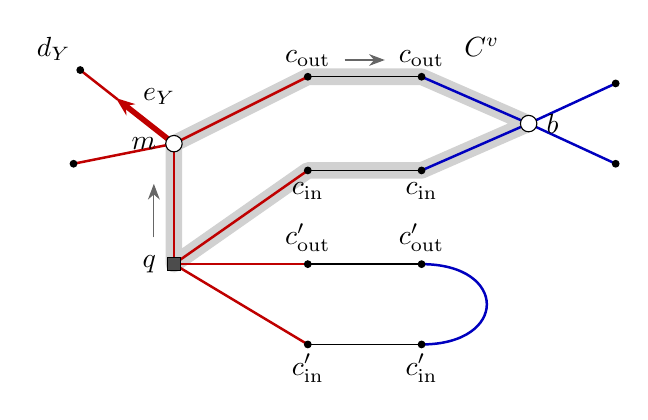
\begin{tikzpicture}[scale=0.85,
  leaf/.style={circle,fill=black,inner sep=1.0pt},
  pv/.style={circle,draw=black,fill=white,inner sep=2.1pt},
  qv/.style={rectangle,draw=black,fill=black!70,inner sep=2.4pt},
  redt/.style={draw=red!75!black,line width=0.9pt},
  bluet/.style={draw=blue!75!black,line width=0.9pt},
  joinedge/.style={draw=black,line width=0.5pt},
  markcyc/.style={draw=black!18,line width=6pt,line cap=round,line join=round}]
  \coordinate (m) at (0,1.3);   \coordinate (q) at (0,-0.5);
  \coordinate (or) at (2,2.3);  \coordinate (ir) at (2,0.9);
  \coordinate (opr) at (2,-0.5);\coordinate (ipr) at (2,-1.7);
  \coordinate (dl) at (-1.4,2.4);\coordinate (pl) at (-1.5,1.0);
  \coordinate (ob) at (3.7,2.3); \coordinate (ib) at (3.7,0.9);
  \coordinate (b) at (5.3,1.6);  \coordinate (x1) at (6.6,2.2);
  \coordinate (x2) at (6.6,1.0); \coordinate (opb) at (3.7,-0.5);
  \coordinate (ipb) at (3.7,-1.7);
  \draw[markcyc] (ir) -- (q) -- (m) -- (or) -- (ob) -- (b) -- (ib) -- cycle;
  \draw[redt] (m) -- (or); \draw[redt] (m) -- (pl); \draw[redt] (m) -- (q);
  \draw[redt] (q) -- (ir); \draw[redt] (q) -- (opr); \draw[redt] (q) -- (ipr);
  \draw[redt,line width=2pt,-{Stealth[length=2.4mm]}] (m) -- ($(m)!0.62!(dl)$);
  \draw[redt] ($(m)!0.6!(dl)$) -- (dl);
  \draw[bluet] (b) -- (ob); \draw[bluet] (b) -- (ib);
  \draw[bluet] (b) -- (x1); \draw[bluet] (b) -- (x2);
  \draw[bluet] (opb) .. controls (5.0,-0.5) and (5.0,-1.7) .. (ipb);
  \draw[joinedge] (or) -- (ob); \draw[joinedge] (ir) -- (ib);
  \draw[joinedge] (opr) -- (opb); \draw[joinedge] (ipr) -- (ipb);
  \draw[-{Stealth[length=2mm]},black!60] (2.55,2.55) -- (3.15,2.55);
  \draw[-{Stealth[length=2mm]},black!60] (-0.3,-0.1) -- (-0.3,0.7);
  \node[pv] at (m) {}; \node[qv] at (q) {}; \node[pv] at (b) {};
  \foreach \p in {or,ir,opr,ipr,dl,pl,ob,ib,x1,x2,opb,ipb} \node[leaf] at (\p) {};
  \node[left=3pt] at (m) {$m$}; \node[left=3pt] at (q) {$q$};
  \node[right=3pt] at (b) {$b$}; \node[above left=0pt] at (dl) {$d_Y$};
  \node[above] at (or) {$c_{\mathrm{out}}$}; \node[below=1pt] at (ir) {$c_{\mathrm{in}}$};
  \node[above=1pt] at (opr) {$c'_{\mathrm{out}}$}; \node[below] at (ipr) {$c'_{\mathrm{in}}$};
  \node[above] at (ob) {$c_{\mathrm{out}}$}; \node[below=1pt] at (ib) {$c_{\mathrm{in}}$};
  \node[above=1pt] at (opb) {$c'_{\mathrm{out}}$}; \node[below] at (ipb) {$c'_{\mathrm{in}}$};
  \node at (-0.22,2.0) {$e_Y$}; \node at (4.6,2.75) {$C^v$};
\end{tikzpicture}
\caption{A doubled graph $\mathcal D_v$, $v$ on common cycles $C,C'$ in one
red block. Left: the red tree, with a P-vertex $m$ (circle) and a Q-vertex
$q$ (square). Right: the blue tree of $B_2(C)$ and that of $B_2(C')$, a
single edge. Thin black edges are joining edges; leaves are labelled by
their darts at $v$. The marked cycle $C^v$ (shaded) runs from $c_{\mathrm{in}}$
to $c_{\mathrm{out}}$ in red and back in blue; $C'^v$ also passes through $q$.
The median of $c_{\mathrm{out}},c_{\mathrm{in}},d_Y$ is $m$, so the lobe
attached by $d_Y$ is read by the observer of $(C^v,m,e_Y)$.}
\label{fig:v4-doubled}
\end{figure}

\subsection{Legality}\label{sec:v4-cmp-legal}

\begin{lemma}[anchor paths]\label{lem:v4-anchorpaths}
Let $C\ni v$ be a common cycle and $B=B_i(C)$. (a) $\pi^i_C(v)$ passes through
$\mu_v$ if and only if $\mu$ displays $C$, and then uses the directions whose
expansions contain the edges of $C$ at $v$ (the anchors, for a P node).
(b) For a common cycle $C'\ne C$ through $v$ with $B_i(C')=B$, the paths
$\pi^i_C(v)$, $\pi^i_{C'}(v)$ share no edge and no copy of a P node.
\end{lemma}

\begin{proof}
By Lemma~\ref{lem:v4-frontier}(a) the leaves behind a direction $e$ are the
edges of $B_e$ at $v$, and $B_e$ meets the rest of $B$ only in its poles
by~\ref{it:v4-T1}. (a) The path passes through $\mu_v$ if and only if the
edges of $C$ at $v$ lie behind distinct directions. If both lie in one $B_e$
but $C\not\subseteq B_e$, the paths formed by $E(C)\cap E(B_e)$ have two
distinct ends each, all poles other than $v$, which is impossible; so this
happens exactly when $\mu$ displays $C$. The anchors are those of
Lemma~\ref{lem:v4-display}(a). (b) Leaf edges are darts, distinct for
distinct cycles. An inner edge corresponds to a direction $e$ with poles
$v,w\ne v$; if $\pi^i_C(v)$ uses it, exactly one edge of $C$ at $v$ lies in
$B_e$, so $C$ leaves $B_e$ at $w$ and $w\in V(C)$. If both paths used it, $C,C'$
would share $v,w$. A P node on both would display both,
contradicting Lemma~\ref{lem:v4-display}(b).
\end{proof}

\begin{lemma}[legality]\label{lem:v4-legal}
$\mathcal I$ is a canonical instance; its Q-vertices have degree at least
three and its pipe ends degree at least four. A copy of a free P node lies on
a marked cycle if and only if the node displays a common cycle, and then both
copies do and the pipe is aligned.
\end{lemma}

\begin{proof}
$G$ is simple. Copies of P and R nodes have degree at least three
(Lemma~\ref{lem:v4-frontier}(a)), and a free P node gives a pipe between two
P-vertices of degree at least four in $\mathcal D_p\ne\mathcal D_{p'}$; every
copy has one source, so it lies in at most one pipe. \ref{it:v4-M1}: $C^v$
consists of paths between distinct leaves of a red and of a blue tree and two
distinct joining edges, so it is a directed simple cycle. \ref{it:v4-M2},~\ref{it:v4-M3}: marked cycles at
distinct vertices lie in disjoint doubled graphs; at one vertex, distinct
cycles have distinct leaves and joining edges, and by
Lemma~\ref{lem:v4-anchorpaths}(b) their anchor paths share only copies of
flip nodes, which are Q-vertices.

\ref{it:v4-M4}: let $\mu$ be a free P node with poles $p,p'$ in $B$ of colour
$i$. Marked cycles through $T_B(p)$ use only paths $\pi^i_C(p)$ with
$B_i(C)=B$, so by Lemma~\ref{lem:v4-anchorpaths}(a) $\mu_p$ is on a marked
cycle if and only if $\mu$ displays a common cycle. If it displays none, the
pipe is off. Otherwise it displays exactly one, $C$
(Lemma~\ref{lem:v4-display}(b)); then $p,p'\in V(C)$ and $B=B_i(C)$, so
$\mu_p\in C^p$ and $\mu_{p'}\in C^{p'}$, with anchors the darts of
$\{\varepsilon^{\mathrm{out}}_p,\varepsilon^{\mathrm{in}}_p\}=
\{\varepsilon^{\mathrm{in}}_{p'},\varepsilon^{\mathrm{out}}_{p'}\}$
(Lemma~\ref{lem:v4-display}(c)); $\varphi_\mu$ preserves directions, so the
pipe is aligned.

Reads: $d_Y$ is not a dart of $C$, so by Lemma~\ref{lem:v4-median}(e) $m_Y$ is
an inner node of $\pi^i_C(a_Y)\subseteq C^{a_Y}$ and $e_Y$ differs from its
anchors; so the triple is observable, or $\eta_Y$ is defined. Observers arise
only as $\langle t\rangle$.
\end{proof}

\subsection{Induced rotation systems and reads}\label{sec:v4-cmp-induced}

For an embedding $\mathcal E$ of a relevant block $B$ of colour $i$, the
rotation system \emph{induced} on $T_B(v)$ gives $\mu_v$ the rotation
$\mathcal E_\mu(v)^{(i)}$. For a family $\mathfrak E=(\mathcal E(B))_B$ of
embeddings of the relevant blocks, $\rho^{\mathfrak E}$ is induced on every
tree, and $\beta^{\mathfrak E}(r_\mu)=r_\mu(\mathcal E(B))$.

\begin{lemma}[induced rotation systems]\label{lem:v4-induced}
\leavevmode
\begin{enumerate}[label=(\alph*),nosep]
\item $(\rho^{\mathfrak E},\beta^{\mathfrak E})$
satisfies~\ref{it:v4-W1} and~\ref{it:v4-W2}.
\item If $\rho$ and an assignment $\beta$ of the $r_\mu$
satisfy~\ref{it:v4-W1} and~\ref{it:v4-W2}, there is exactly one $\mathfrak E$
with $\rho=\rho^{\mathfrak E}$, and $\beta=\beta^{\mathfrak E}$; the rotations
of all $\mathcal E(B)$ are computed in $O(N)$ time.
\item $\rho^{\mathfrak E}$ is planar on $\mathcal D_v$ if and only if some
cyclic order $\omega_v$ of the common darts at $v$ restricts to the order of
the common darts of $B$ in $\mathcal E(B)(v)$ for every relevant block $B$ at
$v$ and makes both block partitions noncrossing; it is computed by
Lemma~\ref{lem:v4-partitions}.
\end{enumerate}
\end{lemma}

\begin{proof}
(a) For a P node, $\mathcal E_\mu(p')=\rev\mathcal E_\mu(p)$ on directions
(\ref{it:v4-T3}), so $\rho^{\mathfrak E}(\mu_{p'})=\rev\varphi_\mu
(\rho^{\mathfrak E}(\mu_p))$ in both colours, which is~\ref{it:v4-W1} for free
$\mu$. At a copy of a flip node, $\rho^{\mathfrak E}(\mu_v)$ is $\mathcal
R_\mu(v)^{(i)}=\psi(\mu_v)$ or its reverse according to $r_\mu$,
which is~\ref{it:v4-W2}.

(b) Embed every R skeleton by $\mathcal R_\mu$ or its mirror image according
to $\beta(r_\mu)$, and every P skeleton by the order $\rho(\mu_p)^{(i)}$ at
$p$. The order at $p'$ is its reverse: for free $\mu$ by~\ref{it:v4-W1}; with
three skeleton edges because $\psi(\mu_{p'})=\rev\varphi_\mu(\psi(\mu_p))$,
both copies follow the same colour convention and share the flip $r_\mu$,
so~\ref{it:v4-W2} gives $\rho(\mu_{p'})=\rev\varphi_\mu(\rho(\mu_p))$.
So the rotations $\rho(\mu_v)^{(i)}$ are consistent in the sense of
Lemma~\ref{lem:v4-trees}(b) (at R nodes by~\ref{it:v4-W2}), which gives a
unique $\mathcal E(B)$ inducing them, with rotation at $v$ the frontier of $T_B(v)$; by (a)
and~\ref{it:v4-W2}, $\beta(r_\mu)=r_\mu(\mathcal E(B))$ for all flip nodes.

(c) Inner tree nodes have all darts in their tree, and a leaf has at most one
further dart, a joining edge to a leaf of another tree. The frontier of a red tree under
$\rho^{\mathfrak E}$ is $\mathcal E(B)(v)$ (Lemma~\ref{lem:v4-frontier}(b)),
that of a blue tree its reverse (Lemma~\ref{lem:v4-median}(c)). Contracting
all trees preserves genera (Lemma~\ref{lem:v4-median}(d)) and gives the
bipartite multigraph of Lemma~\ref{lem:v4-partitions} on the relevant blocks
at $v$, with rotation $\sigma_B$ at red and $\rev\sigma_B$ at blue blocks,
$\sigma_B$ the order of the common darts of $B$ in $\mathcal E(B)(v)$, plus
isolated vertices from trees without joining edges. Apply that lemma.
\end{proof}

\begin{lemma}[read values]\label{lem:v4-readval}
Let $Y$ be a lobe of $C$ in colour $i$, $B=B_i(C)$, $\mathcal E$ an embedding
of $B$, and $(\rho,\alpha)$ satisfy~\ref{it:v4-W2},~\ref{it:v4-W3}, with
$\rho$ induced by $\mathcal E$ on $T_B(a_Y)$. Then
\[
\alpha(y_Y)\oplus\eta_Y=\gap_\rho(C^{a_Y},m_Y,e_Y)
=\gap_{\mathcal E}(C,a_Y,d_Y)=\side_{\mathcal E}(C,Y).
\]
\end{lemma}

\begin{proof}
Write $a=a_Y$, $m=m_Y$ with source $\mu$, and $e_{\mathrm{out}},
e_{\mathrm{in}}$ for its darts towards the leaves of $c_{\mathrm{out}}(C,a)$,
$c_{\mathrm{in}}(C,a)$. First equality: \ref{it:v4-W3} for a P-vertex;
\ref{it:v4-W2} and Lemma~\ref{lem:v4-gaps}(a) for a Q-vertex, which has
degree at least three. Second: for $i=1$, $C^a$ leaves $m$ by
$e_{\mathrm{out}}$ and enters by $e_{\mathrm{in}}$, and $\rho(m)=\mathcal
E_\mu(a)$, so the gap is $\operatorname{or}_{\mathcal E_\mu(a)}
(e_{\mathrm{out}},e_Y,e_{\mathrm{in}})$; for $i=2$ the traversal and the
rotation are both reversed, giving $\operatorname{or}_{\rev\mathcal E_\mu(a)}
(e_{\mathrm{in}},e_Y,e_{\mathrm{out}})$, the same value. As the frontier of
$T_B(a)$ under $\mathcal E$ is $\mathcal E(a)$, Lemma~\ref{lem:v4-median}(e)
turns this into $\operatorname{or}_{\mathcal E(a)}(c_{\mathrm{out}}(C,a),d_Y,
c_{\mathrm{in}}(C,a))=\gap_{\mathcal E}(C,a,d_Y)$. Third: Lemma~\ref{lem:v4-sector} for the edge $ax_Y$.
\end{proof}

\subsection{Equivalence, size and construction time}\label{sec:v4-cmp-equiv}

\begin{theorem}[compilation]\label{thm:v4-compile}
For a normalized instance $(G_1,G_2)$ and its compiled instance $\mathcal I$:
(a) from every witness of $\mathcal I$ a SEFE is computed in $O(N^2)$ time;
(b) from every SEFE, given by its embeddings, a witness of $\mathcal I$ is
computed in $O(N^2)$ time; (c) $|\mathcal I|=O(N)$, and $\mathcal I$ is
built in $O(N^2)$ time. In particular, $(G_1,G_2)$ has a SEFE if and only if
$\mathcal I$ is feasible.
\end{theorem}

\begin{proof}
(a) Let $(\rho,\alpha)$ be a witness. Lemma~\ref{lem:v4-induced}(b) gives
$\mathfrak E$ with $\rho=\rho^{\mathfrak E}$: R nodes are embedded by their
flips, P nodes by the rotation at either copy, reversed in blue trees. Embed
the other blocks arbitrarily, and let $s(C,Z)=\alpha(s_{C,Z})$ where defined
and $0$ otherwise. \ref{it:v4-R1}: $\rho$ is planar on every $\mathcal D_v$,
so Lemma~\ref{lem:v4-induced}(c) gives $\omega_v$; other blocks have no
common darts. \ref{it:v4-R2}: $x\in V(B_i(C))\setminus V(C)$ lies in a lobe
$Y$ inside the component $Z\ni x$ of $U-V(C)$, and by
Lemma~\ref{lem:v4-readval} and the row of $Y$,
$\side_{\mathcal E(B_i(C))}(C,x)=\alpha(y_Y)\oplus\eta_Y=\alpha(s_{C,Z})=
s(C,x)$. Theorem~\ref{thm:v4-repair} gives a SEFE restricting to $\mathcal
E(B)$ on every block. Time: $O(N)$ for $\mathfrak E$, the other
blocks~\cite{HT74} and all $\omega_v$; $O(N)$ per common cycle for $\mathcal
Z_C$; $O(N^2)$ for the repair.

(b) By Lemma~\ref{lem:v4-necessary} the block restrictions and the sides of
the components form a block datum satisfying~\ref{it:v4-R1},~\ref{it:v4-R2}.
Put $\rho=\rho^{\mathfrak E}$ for the relevant blocks, $\alpha(r_\mu)=
r_\mu(\mathcal E(B))$, $\alpha(x)=\gap_\rho(\operatorname{obs}(x))$ for
observers and $\alpha(s_{C,Z})=s(C,Z)$. Then~\ref{it:v4-W1},~\ref{it:v4-W2}
hold by Lemma~\ref{lem:v4-induced}(a), \ref{it:v4-W3} by definition, planarity
by~\ref{it:v4-R1} and Lemma~\ref{lem:v4-induced}(c), and the row of a lobe
$Y\subseteq Z$ by Lemma~\ref{lem:v4-readval} and~\ref{it:v4-R2}. Time: an
inner node $x$ of $T_B(v)$ is the median of any three leaves behind distinct
darts of $x$, so by Lemma~\ref{lem:v4-median}(e) $\rho^{\mathfrak E}(x)$ is
the order in $\mathcal E(B)(v)$ of one leaf behind each dart, reversed in
blue trees; this is $O(t)$ per node of a tree with $t$ nodes, $O(N^2)$ in
all. Flips, observers and reads cost $O(N)$ each, and $\alpha(s_{C,Z})$ can
be taken as the value of any read in $Z$, so the sides need not be computed.

(c) \emph{Size.} $T_B(v)$ has at most $2\deg_B(v)$ nodes
(Lemma~\ref{lem:v4-frontier}(a)), so the trees have at most
$4(|E_1|+|E_2|)$ nodes; there are $2|E(H)|$ joining edges. Marked cycles are
edge-disjoint, and every dart belongs to at most one reference or pipe, so
cycles, references and bijections have total length $O(|E(G)|)$. There are at
most $|Q|$ flips, and at most $2(|E_1|+|E_2|)$ lobes, each giving at most one
observer, side variable and row.

\emph{Time.} Blocks, SPQR trees, reference embeddings and all trees with the
copies of every node take linear time (\cite{Tar72,HT73,HT74,GM01},
Lemma~\ref{lem:v4-trees}), and yield the Q-cells and pipes. An anchor path
takes $O(\deg_{G_i}(v))$ by search, $O(\sum_v\deg_H(v)\deg_U(v))=O(N^2)$ in
all. For each of at most $N$ common cycles, lobes, attachment edges and
$\mathcal Z_C$ take $O(N)$. For each of at most $2|E(H)|$ pairs $(C,a)$, $a$
an attachment vertex, one search of $T_{B_i(C)}(a)$ from $\pi^i_C(a)$ gives
every leaf its median with the leaves of $C$ and the dart towards it, in
$O(\deg_{G_i}(a))$; an offset $\eta_Y$ takes $O(\deg m_Y)$. Storing observers
at the darts of their P-vertices keeps $\mathcal I$ canonical.
\end{proof}

\section{The local-gap engine}\label{sec:eng4}

\providecommand{\obs}{\operatorname{obs}}
\newcommand{\anout}{c_{\mathrm{out}}}
\newcommand{\anin}{c_{\mathrm{in}}}

The input of this section is an instance $\mathcal I$
(Definition~\ref{def:v4-instance}); the output is a rejection if $\mathcal I$
is infeasible, and otherwise a system of binary rows whose solutions,
restricted to $X$, are exactly $F(\mathcal I)$, with a witness for every
solution (Theorem~\ref{thm:eng4-main}). Witnesses, the contract, relocation
and the observers $\langle t\rangle$ are those of Section~\ref{sec:v4-lang}.
We use Lemma~\ref{lem:v4-gaps}(a),(b); the proof of (b) uses only
$\rho_{v'}=\rev\varphi(\rho_u)$ and that $\varphi$ maps the anchor pair at
$u$ onto that at $v'$, so we apply it also to such bijections that are not
pipes.

The engine runs the Synchronized Planarity algorithm of Bl\"asius, Fink and
Rutter~\cite{BFR21} (numbers refer to arXiv:2007.15362v2), with its graph
operations unchanged up to subdividing the edges at the leaves of the trees
inserted by PropagatePQ, and carries observations and rows along. Our pipe
condition $\rho_v=\rev\varphi(\rho_u)$ is that of~\cite{BFR21}. The
equivalence lemmas of~\cite{BFR21} concern feasibility of the bare instance,
whereas the contract preserves the feasible assignments of all existing
variables; so all statements about observations are proved here. We use
unchanged: the operations of~\cite[Sections~3.1.1--3.4]{BFR21}; splits and
joins along pipes~\cite[Section~2, Lemma~1]{BFR21}; the schedule in the
proof of~\cite[Lemma~7]{BFR21}; the potential of~\cite[Section~3.6]{BFR21} with~\cite[Lemma~9, Lemma~10(i), Lemma~11]{BFR21};
and that a wheel lies in one rigid skeleton~\cite[proof of Lemma~8]{BFR21}.
The relation to the rotation variables and triple equations
of~\cite[Chapter~8]{Pfr22} is discussed in the introduction.

\subsection{Wheels, embedding trees and Q-intersections}\label{sec:eng4-wheels}

The \emph{wheel graph} $G^W$ replaces every Q-vertex $q$ with $\deg q\ge3$
by a wheel~\cite[Section~2]{BFR21}: each edge $e$ at $q$ is subdivided by a
\emph{port} next to $q$ (twice if both ends are such Q-vertices), and the
ports are joined by a \emph{rim} in the order $\psi(q)$; $q$ is the
\emph{hub}. The neighbours of a hub are exactly its ports, pairwise distinct,
and its rim is a simple cycle. Darts of $G$ correspond to darts of $G^W$ at
the same vertex, and a marked cycle $C$ is \emph{lifted} to $C^W$ through the
spokes and ports of the hubs it passes, with the same anchors at P-vertices.

\begin{lemma}[wheels]\label{lem:eng4-wheel}
(a) Every planar $\rho$ of $G$ with $\rho_q\in\{\psi(q),\rev\psi(q)\}$ for
all hubs extends to a planar $\rho^W$ of $G^W$ with the same rotations at all
vertices of $G$. (b) Deleting the rims of a planar $\rho^W$ and suppressing
the ports gives a planar $\rho$ of $G$ with the same rotations at vertices of
$G$ and $\rho_q\in\{\psi(q),\rev\psi(q)\}$ at every hub. (c) A P-vertex is a
cutvertex of $G$ if and only if it is one of $G^W$. (d)
$\gap_\rho(C,v,d)=\gap_{\rho^W}(C^W,v,d)$ for every observable triple.
\end{lemma}

\begin{proof}
(a) Draw each rim on a small circle around its hub. (b) The wheel is $3$-connected, so the restriction of $\rho^W$ to it is one
of its two mirror embeddings, and the rotation at the hub is the rim order
$\psi(q)$ or its reverse. (c) Contracting the wheels of $G^W-w$ gives $G-w$. (d)
The rotation and the anchors at $v$ are the same.
\end{proof}

\paragraph{SPQR trees and embedding trees.} For a block $B$ of $G^W$ that is
neither an edge nor a cycle we use from Section~\ref{sec:v4-spqr}
\ref{it:v4-T1}--\ref{it:v4-T4}, reflection bits $r_\mu$, displayed cycles,
anchors and gaps $\gap_\mu$ of P skeletons (Lemma~\ref{lem:v4-display}),
embedding trees $\Theta_B(v)$ with frontiers, local reads and their complete
family (Lemmas~\ref{lem:v4-frontier}, \ref{lem:v4-trees}); and
Lemmas~\ref{lem:v4-median} and~\ref{lem:v4-assembly}. The \emph{embedding tree} $T_v$
of~\cite[Section~2]{BFR21} is $\Theta_B(v)$ with every P node of degree three
read as a Q node; it is \emph{trivial} if it is a single P node.

\begin{lemma}[Q-intersections]\label{lem:eng4-qint}
Let $q$ be a hub of $G^W$ and $B$ its block.
\begin{enumerate}[label=(\alph*),nosep]
\item $q$ is not a cutvertex of $G^W$.
\item $q$ is not a pole of a P node of $\mathcal T_B$.
\item Both poles of a P node with at least four skeleton edges are
  P-vertices of $G$.
\item Distinct lifted marked cycles meet only at hubs. Hence no cutvertex of
  $G^W$ lies on two lifted marked cycles, and at most one lifted marked cycle
  passes through both poles of a P node.
\end{enumerate}
\end{lemma}

\begin{proof}
(a) The rim connects all neighbours of $q$ in $G^W-q$. (b) Let $\mu$ have
poles $q,w$. The ports other than $w$ are inner to expansions, and the rim
minus $w$ is connected and avoids $q,w$; so they and their spokes lie in one
expansion, and at most the spoke $qw$ lies in another. So at most two
expansions contain darts at $q$, but $\mu$ has at least three skeleton
edges. (c) A pole $a$ has at least four darts, so it is not a Q-vertex of
degree at most two, nor a hub by (b). Let $a$ be a port of the hub $q$, with
rim neighbours $p',p''$; by (b) the other pole $b$ is not $q$. If
$b\notin\{p',p''\}$, the spoke and both rim edges at $a$ end in vertices
joined in $G^W-\{a,b\}$ through $q$; if $b=p'$, the spoke and $ap''$ end at
$q,p''$, joined by a spoke. Either way at most three expansions contain
darts at $a$, a contradiction. (d) Two marked cycles share only Q-vertices
and no edge; a Q-vertex of degree at most two or a port lies on at most one
lift. So shared vertices of lifts are hubs, neither cutvertices (a) nor
poles (b).
\end{proof}

\subsection{The operations}\label{sec:eng4-ops}

Each lemma below states that a step satisfies the contract and that its output is an instance, in
particular satisfies~\ref{it:v4-M1}--\ref{it:v4-M4}. Throughout,
$(u,v,\varphi)$ is the pipe acted on, $D=\deg u$, and observers are created
as $\langle t\rangle$. Old rows are kept, so it suffices to check planarity,
\ref{it:v4-W1}--\ref{it:v4-W3} and the new rows. Rotations change only at
the vertices acted on and, in SimplifyMatching, at the partner pole.



\begin{lemma}[ConvertSmall]\label{lem:eng4-convert}
Let $u$ be a P-vertex with $\deg u\le3$. Make $u$ a Q-vertex with any
reference $\psi(u)$ and a fresh flip $g=f(u)$. If $u$ is matched by
$(u,v,\varphi)$, delete the pipe and make $v$ a Q-vertex of the same Q-cell,
$f(v)=g$, with $\psi(v)=\rev\varphi(\psi(u))$. Relocate every observer of
$(C,z,d)$, $z\in\{u,v\}$, to $g\oplus\gap_{\psi(z)}(C,z,d)$. This step
satisfies the contract with $\rho'=\rho$ and yields an instance.
\end{lemma}

\begin{proof}
The invariant is clear. Observations at $z$ need $\deg z=3$. Forward: put
$\alpha'(g)=1$ if and only if $\deg u=3$ and $\rho_u=\rev\psi(u)$; then
$\rho_v=\rev\varphi(\rho_u)$ is $\psi(v)$ or $\rev\psi(v)$ accordingly,
and Lemma~\ref{lem:v4-gaps}(a) gives the new rows. Backward: for $\deg u=3$,
\ref{it:v4-W2} gives $(\rho_u,\rho_v)=(\psi(u),\rev\varphi\psi(u))$ or
$(\rev\psi(u),\varphi\psi(u))$, so the pipe holds (trivially if $\deg u\le2$),
and relocated observations hold by the same identity.
\end{proof}

\paragraph{Encapsulation.} Let $u$ be a P-vertex that is a cutvertex of its
component $W$, and $Y_1,\dots,Y_k$ the components of $W-u$.
As in~\cite[Section~3.2]{BFR21}, for $j=1,\dots,k$ split the component of
$u$ along the cut $(V(Y_j),\text{rest})$, creating the \emph{residual cap}
$u_j$ (contracted rest), the \emph{ray} $u'_j$ (contracted $Y_j$) and the cap
pipe $(u_j,u'_j,\chi_j)$. An edge $e=uy$, $y\in Y_j$, becomes a \emph{star
edge} $uu'_j$, which keeps the dart of $e$ at $u$, and a \emph{residual edge}
$u_jy$, which keeps the dart at $y$; so old vertices keep their dart sets and
rotations. The component of $u$ becomes the star $S_u$. If $u\in
C\in\mathcal M$, the anchors of $u$ end in one $Y_{j_0}$; with $\hat
u=u'_{j_0}$, $C$ is replaced by $C^{\mathrm{res}}$ through $u_{j_0}$ and
the residual edges, and the \emph{star digon} $C^\star_u:u\to\hat u\to u$
(out along the star edge of $\anout(C,u)$, back along that of $\anin(C,u)$)
is added. Observations at $u$ now refer to $C^\star_u$, with the same dart;
those at other vertices of $C$ to $C^{\mathrm{res}}$.

\begin{lemma}[encapsulation]\label{lem:eng4-encap}
The encapsulation satisfies the contract with rotations unchanged at all old
vertices, and its result is an instance. A vertex $y\ne u$ of $W$ is a
cutvertex of $W$ if and only if it is one of the piece $Y_j+u_j$
containing it, and every residual cap is a block-vertex of its piece.
\end{lemma}

\begin{proof}
Both shores of each cut are connected, so by~\cite[Lemma~1, Section~2]{BFR21}
every planar rotation system splits into a planar one with the same old
rotations satisfying the cap pipes, and conversely the joins along the cap
pipes are planar and keep old rotations. Observations keep their values,
as rotations and anchors are unchanged.
\emph{Invariant.} $C^{\mathrm{res}}$ and $C^\star_u$ are simple, the new
vertices on them lie on one marked cycle each, $u$ lies only on
$C^\star_u$, and other marked cycles are unchanged. The cap pipe at $j_0$
maps anchors to anchors, hence is aligned; a marked cycle through $u_j$ or
$u'_j$, $j\ne j_0$, would cross the $j$-th cut, so the other cap pipes are
off. \emph{Cutvertices.} The components of $W-y$ avoiding $u$ lie in $Y_j$
and survive in $(Y_j+u_j)-y$, and $u_j$ lies in another one. Conversely, if
$W-y$ is connected, every component of $Y_j-y$ is adjacent to $u$, hence to
$u_j$. Finally $(Y_j+u_j)-u_j=Y_j$ is connected.
\end{proof}

\paragraph{Joining two stars.}
Let $S_u,S_v$ be disjoint stars (parallel edges allowed) with centres $u,v$
and ray sets $R_u,R_v$, and let $\varphi:A_u\to A_v$ be a bijection. For
$d\in A_u$ let $r(d)\in R_u$ be the ray at the other end of $d$, and
$r'(d')\in R_v$ likewise for $d'\in A_v$. The
\emph{join}~\cite[Section~2]{BFR21} deletes $u$ and $v$ and adds, for every
$d\in A_u$, an edge $\ell_d=r(d)\,r'(\varphi d)$ that takes over the ray
darts of $d$ and $\varphi(d)$. The result is the bipartite \emph{ray graph}
$K$; a rotation of a ray is read in $S_u\cup S_v$ and in $K$ alike, darts
renamed.

\begin{lemma}[stars]\label{lem:eng4-stars}
\begin{enumerate}[label=(\alph*),nosep]
\item A rotation system of two vertices joined by $k\ge1$ parallel edges is
  planar if and only if the rotation of one vertex is the reverse of that of
  the other, edges identified.
\item Let $\sigma$ be a cyclic order of $A_u$ and $\rho'$ rotations of the
  rays. If the rotation system of $S_u\cup S_v$ given by $\sigma$ at $u$,
  $\rev\varphi(\sigma)$ at $v$ and $\rho'$ at the rays is planar, then so
  is $\rho'$ on $K$.
\item Conversely, if $\rho'$ is a planar rotation system of $K$ and $K_j$ is
  a component of $K$, there is a cyclic order $\sigma_j$ of
  $\{d:\ell_d\in K_j\}$ such that the stars $S^j_u,S^j_v$ spanned by these
  darts and by their images, with centre orders $\sigma_j$,
  $\rev\varphi(\sigma_j)$ and $\rho'$ at the rays, are planar; it is
  computable in $O(|E(K_j)|)$ time.
\end{enumerate}
\end{lemma}

\begin{proof}
(a) Read the rotations $\sigma,\pi$ as cyclic permutations of the $k$
edges. A facial walk leaving the first vertex along $e$ leaves it next along
$\sigma\pi(e)$, so facial walks correspond to cycles of $\sigma\pi$. By
Euler's formula the system is planar if and only if there are $k$ of them,
that is, $\sigma\pi=\mathrm{id}$, or $\pi=\rev\sigma$.

(b), (c) The blocks of a star are the bonds between its centre and its rays.
By (a) and Lemma~\ref{lem:v4-assembly}(a),(c), the rotation system of
$S_u\cup S_v$ described in (b) is planar if and only if: every ray $x\in
R_u$ has the rotation $\rev(\sigma|_x)$, where $\sigma|_x$ is the
restriction of $\sigma$ to the darts ending at $x$; every ray $y\in R_v$ has
the rotation $\rev\bigl(\rev\varphi(\sigma)|_y\bigr)$, which is $\sigma|_y$
after identifying the dart of $\ell_d$ at $y$ with $d$; and the partitions
of $A_u$ by $r$ and by $r'\circ\varphi$ are noncrossing in $\sigma$. Put
$\omega=\rev\sigma$. The condition says that $\omega$ restricts to
$\rho'_x$ at every $x\in R_u$ and to $\rev\rho'_y$ at every $y\in R_v$, and
makes both partitions noncrossing. The multigraph of
Lemma~\ref{lem:v4-partitions} for these partitions of $A_u$, with
$\sigma_X=\rho'_x$ at the red blocks $x\in R_u$ and $\sigma_X=\rev\rho'_y$
at the blue blocks $y\in R_v$, is $K$ with the rotation system $\rho'$. So
Lemma~\ref{lem:v4-partitions} gives (b), and, applied to the darts of one
component, (c).
\end{proof}

\paragraph{Gap labels.}
Let $\rho$ be a planar rotation system of $S_u\cup S_v$ with
$\rho_v=\rev\varphi(\rho_u)$, and $\rho'$ its rotations at the rays, which
are planar on $K$ by Lemma~\ref{lem:eng4-stars}(b). Suppose that $a\ne b$
are darts at $u$ with $r(a)=r(b)=:p$ and $r'(\varphi a)=r'(\varphi b)=:q$.
Let $C_u:u\to p\to u$ be the digon that leaves $u$ along $a$ and returns
along $b$, and let
\[
C^\ast:\ p\xrightarrow{\ \ell_b\ }q\xrightarrow{\ \ell_a\ }p .
\]
The \emph{label} of an edge $\ell_d$, $d\ne a,b$, is
$h_d=\gap_\rho(C_u,u,d)$. A ray other than $p$ and $q$ is \emph{ordinary};
all edges at an ordinary ray are labelled. Let $K_0$ be the component of $K$
containing $C^\ast$. For a dart $d\ne a,b$ at $u$ with $\ell_d\in K_0$ define
the \emph{target} $t(d)$: it is $(C^\ast,p,\ell_d)$ if $r(d)=p$; otherwise
$(C^\ast,q,\ell_d)$ if $r'(\varphi d)=q$; otherwise fix a path of $K_0$ from
$r(d)$ that meets $\{p,q\}$ only in its last vertex $z$, let $g$ be its last
edge, and put $t(d)=(C^\ast,z,g)$.

\begin{lemma}[gap labels]\label{lem:eng4-labels}
In this situation:
\begin{enumerate}[label=(\alph*),nosep]
\item the edges at an ordinary ray have one label, as have the edges of a
  component $T\ne K_0$;
\item $\gap_{\rho'}(C^\ast,z,\ell_d)=h_d$ for $z\in\{p,q\}$ and every edge
  $\ell_d\ne\ell_a,\ell_b$ at $z$;
\item every target is an observable triple of $C^\ast$, and
  $\gap_{\rho'}(t(d))=h_d$ for every $d\ne a,b$ with $\ell_d\in K_0$.
\end{enumerate}
\end{lemma}

\begin{proof}
(a) Let $x\in R_u\setminus\{p\}$. The blocks of $S_u$ are the bonds between
$u$ and its rays, so by Lemma~\ref{lem:v4-assembly}(a) the darts at $u$ of
$x$ do not interleave with $a,b$, which belong to $p$. Hence they all lie in
$(a,b)_{\rho_u}$ or all in $(b,a)_{\rho_u}$, and their labels agree. For
$x\in R_v\setminus\{q\}$, likewise the darts at $v$ of $x$ lie all in
$(\varphi a,\varphi b)_{\rho_v}=\varphi((b,a)_{\rho_u})$ or all in
$(\varphi b,\varphi a)_{\rho_v}=\varphi((a,b)_{\rho_u})$, as
$\rho_v=\rev\varphi(\rho_u)$, and the labels agree. A component $T\ne K_0$ avoids
$p$ and $q$, so all its vertices are ordinary, and by connectivity all its
edges have one label.

(b) By Lemma~\ref{lem:eng4-stars}(a), applied to the bond between $u$ and
$p$, the rotation of $p$ is the reverse of the restriction $\sigma$ of
$\rho_u$ to the darts ending at $p$. Now $C^\ast$ leaves $p$ along $\ell_b$
and enters it along $\ell_a$, so for $\ell_d$ at $p$, $d\ne a,b$:
$\ell_d\in(\ell_b,\ell_a)_{\rho'_p}$ if and only if
$d\in(b,a)_{\rev\sigma}=(a,b)_\sigma$, if and only if $d\in(a,b)_{\rho_u}$.
Thus $\gap_{\rho'}(C^\ast,p,\ell_d)=h_d$. At $q$, where $C^\ast$ enters along
$\ell_b$ and leaves along $\ell_a$, symmetrically
$\ell_d\in(\ell_a,\ell_b)_{\rho'_q}$ if and only if $\varphi
d\in(\varphi b,\varphi a)_{\rho_v}=\varphi((a,b)_{\rho_u})$.

(c) If $r(d)=p$ or $r'(\varphi d)=q$, the claim is (b) (and $\ell_d\ne
\ell_a,\ell_b$). Otherwise $r(d)$ is ordinary, the path defining $t(d)$
exists as $K_0$ is connected, and all its vertices except $z$ are ordinary.
Its last edge $g$ has an ordinary end, so $g\ne\ell_a,\ell_b$ and $t(d)$ is
observable. By (a), $\ell_d$ and the first edge of the path have the same
label, and so have any two consecutive edges of the path; so $g$ has label
$h_d$, and (b) gives $\gap_{\rho'}(C^\ast,z,g)=h_d$.
\end{proof}

\begin{figure}[t]
\centering
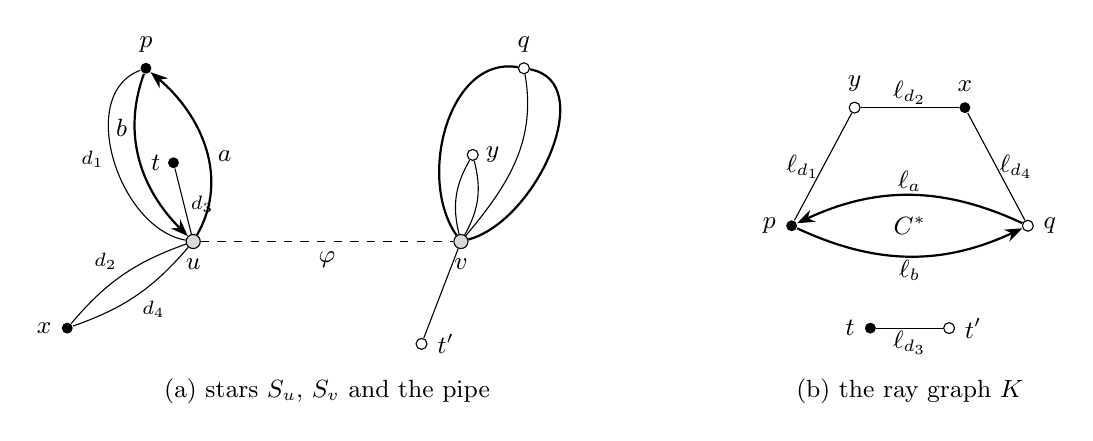
\begin{tikzpicture}[
  every node/.style={font=\small},
  uv/.style={circle,fill=black,inner sep=1.4pt},
  vv/.style={circle,draw=black,fill=white,inner sep=1.4pt},
  ctr/.style={circle,draw=black,fill=black!15,inner sep=1.8pt},
  >={Stealth[length=2.2mm]}]
\begin{scope}
\node[ctr,label=below:$u$] (u) at (0,0) {};
\node[uv,label=above:$p$] (p) at (-0.6,2.2) {};
\node[uv,label={[label distance=-1pt]left:$t$}] (t) at (-0.25,1.0) {};
\node[uv,label=left:$x$] (x) at (-1.6,-1.1) {};
\draw[->,thick] (u) to[out=60,in=-40] node[pos=0.45,right]{$a$} (p);
\draw[->,thick] (p) to[out=250,in=135] node[pos=0.3,left=-1pt]{$b$} (u);
\draw (u) to[out=170,in=200] node[pos=0.5,left]{\scriptsize$d_1$} (p);
\draw (u) -- node[pos=0.45,right=-1pt]{\scriptsize$d_3$} (t);
\draw (u) to[bend right=15] node[pos=0.5,above left=-2pt]{\scriptsize$d_2$} (x);
\draw (u) to[bend left=15] node[pos=0.5,below right=-2pt]{\scriptsize$d_4$} (x);
\node[ctr,label=below:$v$] (v) at (3.4,0) {};
\node[vv,label=above:$q$] (q) at (4.2,2.2) {};
\node[vv,label={[label distance=-1pt]right:$y$}] (y) at (3.55,1.1) {};
\node[vv,label=right:$t'$] (tt) at (2.9,-1.3) {};
\draw[thick] (v) to[out=15,in=-10] (q);
\draw (v) to[out=50,in=-80] (q);
\draw[thick] (v) to[out=125,in=170] (q);
\draw (v) to[bend right=22] (y);
\draw (v) to[bend left=22] (y);
\draw (v) -- (tt);
\draw[dashed] (u) -- node[below]{$\varphi$} (v);
\node at (1.7,-1.9) {(a) stars $S_u$, $S_v$ and the pipe};
\end{scope}
\begin{scope}[xshift=7.6cm]
\node[uv,label=left:$p$] (P) at (0,0.2) {};
\node[vv,label=right:$q$] (Q) at (3,0.2) {};
\node[vv,label=above:$y$] (Y) at (0.8,1.7) {};
\node[uv,label=above:$x$] (X) at (2.2,1.7) {};
\draw[->,thick] (P) to[bend right=25] node[pos=0.5,below,inner sep=1pt]{$\ell_b$} (Q);
\draw[->,thick] (Q) to[bend right=25] node[pos=0.5,above,inner sep=1pt]{$\ell_a$} (P);
\draw (P) -- node[left,inner sep=1pt]{$\ell_{d_1}$} (Y);
\draw (Y) -- node[above,inner sep=1pt]{$\ell_{d_2}$} (X);
\draw (X) -- node[right,inner sep=1pt]{$\ell_{d_4}$} (Q);
\node at (1.5,0.2) {$C^\ast$};
\node[uv,label=left:$t$] (T1) at (1.0,-1.1) {};
\node[vv,label=right:$t'$] (T2) at (2.0,-1.1) {};
\draw (T1) -- node[below,inner sep=1pt]{$\ell_{d_3}$} (T2);
\node at (1.5,-1.9) {(b) the ray graph $K$};
\end{scope}
\end{tikzpicture}
\caption{The join of two stars; filled rays belong to $u$, hollow rays to
$v$, and the drawings realize the rotations. Counter-clockwise around $u$
the darts are $a,d_3,b,d_1,d_2,d_4$. The anchor edges $\ell_a,\ell_b$ form
the digon $C^\ast$. The component $K_0$ contains the bridge of $C^\ast$
through $y$ and $x$, whose edges all have label $1$; this is the local gap
of $\ell_{d_1}$ at $p$ and of $\ell_{d_4}$ at $q$. The detached component
$T=\{tt'\}$ receives the latent bit $h_T=h_{d_3}=0$.}
\label{fig:eng4-join}
\end{figure}

\begin{definition}[EncapsulateAndJoin]\label{def:eng4-ej}
Let $(u,v,\varphi)$ be a pipe whose ends are cutvertices of $G$ (possibly in
one component, possibly adjacent). Encapsulate $u$, then $v$; call the
result $\mathcal I^\ast$, with stars $S_u,S_v$. \emph{Join}
$S_u$ and $S_v$ along the pipe~\cite[Section~3.2]{BFR21}: delete $u$, $v$,
their edges and the pipe, and add the ray graph $K$; the rays keep their cap
pipes. If $K$ is not planar, reject. If the pipe is aligned ($u\in C_u$,
$v\in C_v$), let $a=\anout(C_u,u)$, $b=\anin(C_u,u)$, $p=\hat u$, $q=\hat v$;
replace $C^\star_u$ and $C^\star_v$ by the marked digon $C^\ast:
p\xrightarrow{\ell_b}q\xrightarrow{\ell_a}p$, add a fresh \emph{latent bit}
$h_T$ for every component $T\ne K_0$ of $K$, and relocate every observer of
$(C^\star_u,u,d)$ to $\langle t(d)\rangle\oplus0$ if $\ell_d\in K_0$ and to
$h_T\oplus0$ if $\ell_d\in T$, and every observer of
$(C^\star_v,v,\varphi(d))$ in the same way with offset
$\varepsilon(\varphi)$ in place of $0$.
\end{definition}

\begin{lemma}[EncapsulateAndJoin]\label{lem:eng4-join}
EncapsulateAndJoin satisfies the contract, yields an
instance, and rejects only if $K$ is not planar. It adds $O(D)$ vertices,
edges, pipe incidences, variables and rows.
\end{lemma}

\begin{proof}
By Lemma~\ref{lem:eng4-encap} it suffices to treat $\mathcal
I^\ast\to\mathcal I'$; before the second encapsulation $v$ is still a
cutvertex (of its piece), in the aligned case on the image of $C_v$ with
the same anchors. In
$\mathcal I^\ast$ every observation in the stars is at $u$ or $v$, and in the
aligned case $r(a)=r(b)=p$ and $r'(\varphi a)=r'(\varphi b)=q$, so
Lemma~\ref{lem:eng4-labels} applies with $C_u=C^\star_u$.
\emph{Off pipe.} No observation lies at $u$ or $v$, no marked cycle meets
the stars, and the step is the join of~\cite{BFR21}. Its inverse is the
backward construction below with any component as $K_0$ and any dart $a$ of
it, all other components inserted after $a$; both keep rotations and
anchors at observed vertices. From now on the pipe is aligned.
\emph{Invariant.} $K$ is bipartite and loopless, rays keep their degrees,
$C^\ast$ is a digon on new edges, no other marked cycle meets a ray, the cap
pipes at $p,q$ stay aligned and the others off; targets are observable
(Lemma~\ref{lem:eng4-labels}(c)).
\emph{Forward.} Given a witness $(\rho,\alpha)$ of $\mathcal I^\ast$, let
$\rho'$ consist of its rotations at the rays and $\rho$ elsewhere; it is
planar by Lemma~\ref{lem:eng4-stars}(b), and the cap pipes hold. Give new
observers their gaps and $h_T$ the common label of $T$
(Lemma~\ref{lem:eng4-labels}(a)). The observation of $(C^\star_u,u,d)$ has
value $h_d$, which is $\alpha'(h_T)$ if $\ell_d\in T$ and
$\gap_{\rho'}(t(d))$ if $\ell_d\in K_0$ (Lemma~\ref{lem:eng4-labels}(c)); at
$v$, Lemma~\ref{lem:v4-gaps}(b) gives
$\gap_\rho(C^\star_v,v,\varphi d)=h_d\oplus\varepsilon(\varphi)$.

\emph{Backward.} Given a witness $(\rho',\alpha')$ of $\mathcal I'$,
Lemma~\ref{lem:eng4-stars}(c) gives for every component $K_j$ planar stars
$S^j_u,S^j_v$ with the ray rotations of $\rho'$ and centre orders $\omega_j$,
$\rev\varphi(\omega_j)$. Start with $\rho_u=\omega_0$,
$\rho_v=\rev\varphi(\omega_0)$. For every $T=K_j$, $j\ge1$, insert a linear
order $L_T$ representing $\omega_j$ into $\rho_u$ directly after $a$ if
$\alpha'(h_T)=0$ and directly after $b$ if $\alpha'(h_T)=1$, and
$\rev\varphi(L_T)$ into $\rho_v$ directly before $\varphi(a)$, respectively
$\varphi(b)$; this preserves $\rho_v=\rev\varphi(\rho_u)$. The final
$\rho_u$ restricts to every $\omega_j$, and dart sets of distinct $K_j$ do
not interleave, as each insertion is contiguous. So the bonds of $S_u$ are
planar and pairwise noninterleaving, and $S_u$ is planar by
Lemma~\ref{lem:v4-assembly}(c); likewise $S_v$; the pipes hold. Later
insertions after $a$ or $b$ keep earlier blocks in their interval, so
$\gap_\rho(C^\star_u,u,d)=\alpha'(h_T)$ for $\ell_d\in T$; and they keep
the cyclic order of $\omega_0$, so for $\ell_d\in K_0$,
$\gap_\rho(C^\star_u,u,d)=\gap_{\omega_0}(C^\star_u,u,d)=\gap_{\rho'}(t(d))$
by Lemma~\ref{lem:eng4-labels}(c) for $S^0_u,S^0_v$, whose join is $K_0$.
Observations at $v$ follow by Lemma~\ref{lem:v4-gaps}(b).
\emph{Rejection and size.} The forward construction does not use rows, so a
witness forces $K$ to be planar. The step adds $O(D)$ rays, cap pipes, edges
and targets, at most $D-2$ latent bits and at most $2(D-2)$ relocations.
\end{proof}

\paragraph{PropagatePQ.} Let $u$ be a matched block-vertex whose embedding
tree $T_u$, computed in the block of $G^W$ containing $u$, is not trivial. As
in~\cite[Section~3.3]{BFR21}, replace $u$ by $T_u$: its leaves become
vertices $\ell_d$ adjacent to their inner node and to the other end of $d$
(whose dart there keeps its identity); replace $v$ by a copy $T'_u$ under an
isomorphism $\kappa$, the leaf $\kappa(\ell_d)$ receiving the edge of
$\varphi(d)$ (an edge $uv$ thus joins two leaves); for each inner node
$\alpha$ let $\kappa_\alpha$ map the darts at $\alpha$ to those at
$\kappa\alpha$ (tree darts to tree darts). Add the pipe
$(\alpha,\kappa\alpha,\kappa_\alpha)$ for every P node $\alpha$. For every Q
node $\alpha$ make $\alpha$ and $\kappa\alpha$ Q-vertices of one fresh
Q-cell with a fresh flip $g_\alpha=f(\alpha)=f(\kappa\alpha)$,
$\psi(\alpha)=\theta_\alpha$, the reference order of the
node (either order for a P node of degree three read as a Q node), and
$\psi(\kappa\alpha)=\rev\kappa_\alpha(\theta_\alpha)$. Delete the pipe
$(u,v,\varphi)$. If $u\in C$, replace the visit of $C$ at $u$ by the path of
$T_u$ from $\ell_{\anin(C,u)}$ to $\ell_{\anout(C,u)}$ (the new cycle $C^T$;
observations at other vertices of $C$ now refer to $C^T$, with unchanged
anchors); treat $v$ and $C(v)$ likewise in $T'_u$. \emph{Median transport:}
for an observer $x$ of $(C,u,d)$ let $m$ be the median of
$\ell_{\anout(C,u)},\ell_{\anin(C,u)},\ell_d$ in $T_u$ and $\delta$ the dart
of $m$ towards $\ell_d$; relocate $x$ to $\langle C^T,m,\delta\rangle\oplus0$
if $m$ is a P node and to $f(m)\oplus\gap_{\theta_m}(C^T,m,\delta)$ if $m$ is
a Q node. Observers at $v$ are treated in the same way in $T'_u$.

\begin{lemma}[PropagatePQ]\label{lem:eng4-ppq}
This step satisfies the contract and yields an instance. It adds $O(D)$
vertices, edges, pipe incidences, variables and rows.
\end{lemma}

\begin{proof}
\emph{Invariant.} $C^T$ replaces $u$ by a path of new vertices, which lie on
no other marked cycle. As $\varphi$ maps the anchors of $u$ onto those of
$v$, the path of $C(v)^T$ in $T'_u$ is $\kappa$ of the path $P$ of $C^T$, so
the new pipes are aligned on $P$ and off elsewhere. The median $m$ lies on
$P$, $\delta$ does not, and $C^T$ enters $m$ towards $\ell_{\anin(C,u)}$ and
leaves towards $\ell_{\anout(C,u)}$, so targets are observable.
\emph{Median identity.} If $\rho'$ is planar on $G'$, contracting $T_u$ and
$T'_u$ gives a planar $\rho$ with the frontiers at $u,v$
(Lemma~\ref{lem:v4-median}(d)), and by Lemma~\ref{lem:v4-median}(e)
$\gap_\rho(C,u,d)=\gap_{\rho'}(C^T,m,\delta)$, which is
$f(m)\oplus\gap_{\theta_m}(C^T,m,\delta)$ at a Q node by~\ref{it:v4-W2} and
Lemma~\ref{lem:v4-gaps}(a); likewise at $v$.
\emph{Forward.} By Lemmas~\ref{lem:eng4-wheel}(a)
and~\ref{lem:v4-frontier}(b), $\rho_u$ is the frontier of $T_u$ with the
rotations induced by an embedding of the block. Give $T'_u$ the mirrored
rotations $\rev\kappa_\alpha(\rho'_\alpha)$; its frontier is
$\rev\varphi(\rho_u)=\rho_v$~\cite[proof of Lemma~5]{BFR21}, so by
Lemma~\ref{lem:v4-median}(d) the expansion $\rho'$ is planar; the new pipes
hold, and $\alpha'(g_\alpha)=0$ if and only if $\rho'_\alpha=\theta_\alpha$
satisfies~\ref{it:v4-W2} at $\alpha$ and $\kappa\alpha$. The median
identity gives the rows. \emph{Backward.} Contract the trees; pipes and
Q-cells make them mirror images, so $\rho_v=\rev\varphi(\rho_u)$~\cite[proof
of Lemma~5]{BFR21}, and the median identity gives the observations at $u,v$.
\emph{Size.} $T_u$ has $\le D-2$ inner nodes and $D$ leaves.
\end{proof}

\paragraph{SimplifyMatching: the trivial pole.} In the rest of this
subsection $G^W$ is planar, every P-vertex has degree at least four, $u$ is a
matched block-vertex of $G$ with trivial embedding tree, $D=\deg u$, and $B$
is the block of $G^W$ containing $u$. As $T_u$ is trivial, $\Theta_B(u)$
consists of one P node and $D$ leaves: exactly one P or R node $\mu$ of
$\mathcal T_B$ allocates $u$, it is a P node with $D$ skeleton edges
$\varepsilon_1,\dots,\varepsilon_D$, and the expansion $B_i$ of
$\varepsilon_i$ contains exactly one edge at $u$; let $e_i$ be its dart at
$u$. The other pole $w$ of $\mu$ is the \emph{partner} of $u$. Let $I_i$ be
the set of darts at $w$ of the edges of $B_i$.

\begin{lemma}[trivial pole]\label{lem:eng4-pole}
\begin{enumerate}[label=(\alph*),nosep]
\item $w$ is a P-vertex of $G$; the sets $I_i$ are nonempty and partition
  the darts of $B$ at $w$; so $\deg w\ge D$.
\item Every directed simple cycle of $G^W$ through $w$ but not through $u$
  has its two darts at $w$ in one $I_i$ or in one block other than $B$.
\item If $u\in C\in\mathcal M$, then $w\in C$; the anchors
  $e_a=\anout(C,u)$, $e_b=\anin(C,u)$ satisfy $a\ne b$; $C^W$ is a path of
  $B_a$ from $u$ to $w$ followed by a path of $B_b$ from $w$ to $u$; and
  $\anin(C,w)\in I_a$, $\anout(C,w)\in I_b$.
\item If $\deg w=D$, or if $w$ is a block-vertex of $G$ with trivial
  embedding tree, then $\deg w=D$, every $I_i$ has exactly one element, and
  all darts at $w$ lie in $B$.
\end{enumerate}
\end{lemma}

\begin{proof}
(a) Lemma~\ref{lem:eng4-qint}(c), as $D\ge4$; each expansion is connected
and contains $w$. (b) A cycle lies in one block. If $Z\subseteq B-u$ met
two expansions, a maximal subpath of $Z$ in one of them would have both ends
at $w$, so it would be $Z$. (c) $C^W$ lies in $B$, and its darts at $u$ lie
in distinct expansions. Leaving $u$ along $e_a$ it stays in $B_a$ until it
reaches $w$, and symmetrically it returns through $B_b$; it passes $w$ once.
(d) If $\deg w=D$, the $D$ nonempty disjoint sets $I_i$ exhaust $A_w$. If
$w$ is a block-vertex with trivial embedding tree, $\Theta_B(w)$ is one P
node, which must be $\mu$, with one leaf per direction.
\end{proof}

Let $\rho$ be a planar rotation system of $G$ with
$\rho_q\in\{\psi(q),\rev\psi(q)\}$ for every Q-vertex of degree at least
three, $\rho^W$ its extension (Lemma~\ref{lem:eng4-wheel}(a)), and
$\mathcal E$ the embedding of $B$ induced by $\rho^W$. In $\mathcal E(w)$ the
sets $I_i$ form intervals appearing in the order $\mathcal E_\mu(w)$, and in
$\mathcal E(u)=\rho_u$ the darts $e_i$ appear in the order $\mathcal
E_\mu(u)=\rev\mathcal E_\mu(w)$ by \ref{it:v4-T3}, \ref{it:v4-T4}; so $I_k$
directly follows $I_i$ in $\mathcal E(w)$ if and only if $e_i$ directly
follows $e_k$ in $\rho_u$. Each $I_i$ is an interval of
$\mathcal E(w)=\rho_w|_{B}$ and so has a first dart. The \emph{superblock}
$S_i$ is the interval of $\rho_w$ from the first dart of $I_i$ up to,
excluding, the first dart of the next interval $I_k$, with its linear order.
The superblocks partition $A_w$, $I_i\subseteq S_i$, and the other darts of
$S_i$ belong to blocks other than $B$ (Figure~\ref{fig:eng4-superblock}).

\begin{figure}[t]
\centering
\def\sbToW#1#2{\draw (#1) to[out=0,in=#2] ($(w)+(#2:1.3)$) -- (w);}
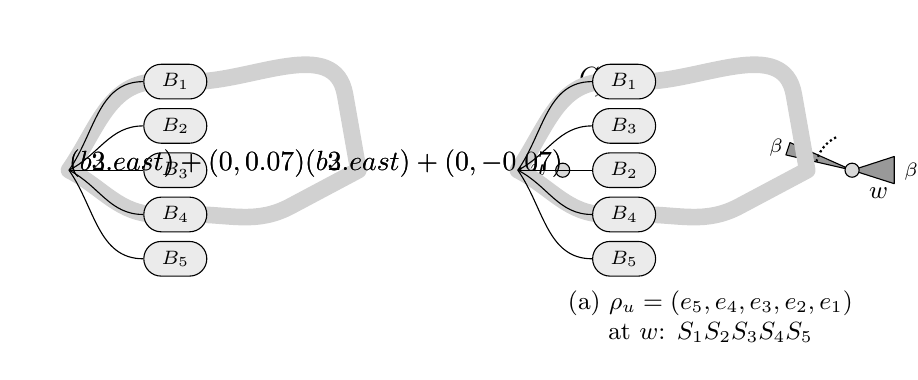
\begin{tikzpicture}[scale=0.75,
  every node/.style={font=\small},
  pole/.style={circle,draw=black,fill=black!15,inner sep=1.8pt},
  bnd/.style={rectangle,rounded corners=2.2mm,draw=black,fill=black!8,
    inner sep=0pt,minimum width=8mm,minimum height=4.4mm,font=\scriptsize},
  oth/.style={draw=black,fill=black!40,line join=round},
  markcyc/.style={draw=black!18,line width=6pt,line cap=round,line join=round},
  >={Stealth[length=2.2mm]}]
\foreach \x/\l/\m/\pa/\pb/\pc/\ps/\pe/\cp/\cw in
  {0/2/3/124/140/156/116/170/{(a) $\rho_u=(e_5,e_4,e_3,e_2,e_1)$}/{$S_1S_2S_3S_4S_5$},
   7.6/3/2/146/162/178/138/192/{(b) $\tau=(e_5,e_4,e_2,e_3,e_1)$}/{$S_1S_3S_2S_4S_5$}} {
\begin{scope}[xshift=\x cm]
\coordinate (u) at (0,0); \coordinate (w) at (4.9,0);
\draw[markcyc] (u) to[out=55,in=180] (1.5,1.5) -- (2.1,1.5) to[out=0,in=100]
  ($(w)+(100:1.3)$) -- (w) -- ($(w)+(208:1.3)$) to[out=208,in=0] (2.1,-0.75)
  -- (1.5,-0.75) to[out=180,in=-27] (u);
\path (1.8,1.5) node[bnd] (b1) {$B_1$} (1.8,0.75) node[bnd] (b2) {$B_\l$}
  (1.8,0) node[bnd] (b3) {$B_\m$} (1.8,-0.75) node[bnd] (b4) {$B_4$}
  (1.8,-1.5) node[bnd] (b5) {$B_5$};
\foreach \b/\a in {b1/55,b2/27,b3/0,b4/-27,b5/-55}
  \draw (u) to[out=\a,in=180] (\b.west);
\sbToW{b1.east}{100} \sbToW{b4.east}{208} \sbToW{b5.east}{240}
\ifnum\l=2 \sbToW{$(b2.east)+(0,0.07)$}{\pa} \sbToW{$(b2.east)+(0,-0.07)$}{\pb}
  \sbToW{b3.east}{180}
\else \sbToW{b2.east}{124}
  \sbToW{$(b3.east)+(0,0.07)$}{\pa} \sbToW{$(b3.east)+(0,-0.07)$}{\pb}
\fi
\filldraw[oth] (w) -- ($(w)+(\pc:1.15)$) -- ($(w)+(\pc+11:1.15)$) -- cycle;
\node[font=\scriptsize,inner sep=1pt,anchor=east] at ($(w)+(\pc+5:1.18)$) {$\beta$};
\filldraw[oth] (w) -- ++(18:0.75) -- ++(270:0.46) -- cycle;
\node[font=\scriptsize,anchor=west] at ($(w)+(0:0.72)$) {$\beta'$};
\draw[densely dotted,thick] ($(w)+(\ps:0.62)$) arc[start angle=\ps,end angle=\pe,radius=0.62];
\draw[->,black!55] (0.55,1.25) -- (0.95,1.5);
\node at (0.45,1.6) {$C$};
\node[pole,label=left:$u$] at (u) {};
\node[pole,label={[label distance=1pt]below right:$w$}] at (w) {};
\node at (2.5,-2.25) {\cp};
\node at (2.5,-2.75) {at $w$: \cw};
\end{scope}}
\end{tikzpicture}
\caption{A trivial pole $u$, its partner $w$ and the five skeleton edges of
$\mu$, drawn as their expansions $B_1,\dots,B_5$; $e_i$ is the dart of
$B_i$ at $u$, the marked cycle $C$ (shaded) runs through $B_1$ and $B_4$,
$\beta,\beta'$ are blocks at $w$ other than $B$, and the drawings realize
the rotations. The superblock $S_2$ (dotted) consists of the darts of $B_2$
and $\beta$ at $w$, and $S_5$ of those of $B_5$ and $\beta'$. Exchanging
$e_2,e_3$ changes only the skeleton embedding of $\mu$ and moves $S_2,S_3$
as wholes; as $e_2,e_3$ stay in $(e_4,e_1)$ at $u$, all gaps at $u$ and $w$
are kept (Lemma~\ref{lem:eng4-superblock}(c)).}
\label{fig:eng4-superblock}
\end{figure}

\begin{lemma}[superblock permutation]\label{lem:eng4-superblock}\label{cor:eng4-fgb}
Let $\rho$ be as above and $\tau$ any cyclic order of $A_u$. Define
$\rho^\tau$ by $\rho^\tau_u=\tau$, $\rho^\tau_z=\rho_z$ for $z\ne u,w$, and
$\rho^\tau_w$ the cyclic concatenation of the superblocks, each with its
linear order, in which $S_k$ directly follows $S_i$ if and only if $e_i$
directly follows $e_k$ in $\tau$.
\begin{enumerate}[label=(\alph*),nosep]
\item $\rho^\tau$ is planar, and $\rho^{\rho_u}=\rho$.
\item If $u$ lies on no marked cycle, every observation has the same value
  under $\rho$ and $\rho^\tau$.
\item If $u\in C\in\mathcal M$ and $\gap_\tau(C,u,e)=\gap_\rho(C,u,e)$ for
  every nonanchor $e$ at $u$, every observation has the same value under
  $\rho$ and $\rho^\tau$.
\end{enumerate}
\end{lemma}

\begin{proof}
(a) $\rho^{\rho_u}=\rho$ was shown above. Let $\mathcal E^\tau$ be the
embedding of $B$ given by \ref{it:v4-T3} with the skeleton embeddings of $\mathcal
E$ except $\mathcal E^\tau_\mu(u)=\tau$. Its rotations are the frontiers of
the embedding trees with the induced node rotations. For $x\in
V(B)\setminus\{u,w\}$, $\mu$ does not allocate $x$, so $\mathcal
E^\tau(x)=\mathcal E(x)$; and $\mathcal E^\tau(u)=\tau$. In $\Theta_B(w)$
only the rotation of $\mu$ changes, to $\rev\tau$; by
Lemma~\ref{lem:v4-median}(b) the contour concatenates the excursions at
$\mu$ in this order, each visiting its leaves in an unchanged order. So
$\mathcal E^\tau(w)$ concatenates the same linear sequences $I_i$, with $I_k$
directly after $I_i$ if and only if $e_i$ directly follows $e_k$ in $\tau$;
this is the restriction of $\rho^\tau_w$ to $B$.

Now apply block assembly (Lemma~\ref{lem:v4-assembly}(c)) to the component
of $u$ in $G^W$, with $\mathcal E^\tau$ on $B$, the restrictions of $\rho^W$
on the other blocks, $\rho^W_x$ at cutvertices $x\ne w$ (where nothing
changed; $u$ is no cutvertex) and $\rho^\tau_w$ at $w$. Every other block
$B'$ at $w$ does not interleave with $B$ in $\rho_w$, so its darts lie in
one \emph{slot} between consecutive darts $g,g'$ of $\mathcal E(w)$. Whether
$g,g'$ lie in one $I_i$ or $g$ ends $I_i$, the whole slot lies in $S_i$
directly after $g$; as superblocks keep their linear order, every slot stays
a contiguous sequence with its old order, followed by a dart of $B$. Hence
$\rho^\tau_w$ restricts to every block rotation at $w$ and no two blocks
interleave. The resulting planar rotation system is $\rho^W$ except at $u,w$;
Lemma~\ref{lem:eng4-wheel}(b) gives $\rho^\tau$.

(b), (c) Rotations and anchors at vertices other than $u,w$ are unchanged,
and observations at $u$ occur only in (c), where the hypothesis applies; so
we consider observations at $w$. (b) A marked cycle $C'$ through $w$ avoids
$u$, so by
Lemma~\ref{lem:eng4-pole}(b) both its anchors at $w$ lie in one $I_i$ or in
one block $B'\ne B$, hence in one superblock $S_i$. For $g\in S_i$ the gap is
determined by the linear order of $S_i$; for $g\notin S_i$,
$g\in(\anout,\anin)$ if and only if $\anin$ precedes $\anout$ in $S_i$. Both
are preserved.

(c) By Lemma~\ref{lem:eng4-pole}(c), $\anin(C,w)\in S_a$ and $\anout(C,w)\in
S_b$ with $a\ne b$. A dart $g\in S_a$ lies in $(\anout(C,w),\anin(C,w))$ if
and only if it precedes $\anin(C,w)$ in $S_a$, and $g\in S_b$ if and only if
it follows $\anout(C,w)$ in $S_b$; these are preserved. For $g\in S_i$, $i\ne
a,b$: $g\in(\anout(C,w),\anin(C,w))$ if and only if $(S_b,S_i,S_a)$ is
counter-clockwise in the order of superblocks, if and only if $(e_a,e_i,e_b)$
is counter-clockwise at $u$ (the superblock order is the reverse of the
order of the $e_j$, for $\rho$ by (a) and for $\rho^\tau$ by definition). So
$\gap(C,w,g)=\gap(C,u,e_i)$ under both systems, equal by hypothesis.
\end{proof}

\begin{lemma}[bond map and orbits]\label{lem:eng4-orbits}
(a) If $\deg w=D$, let $\beta(e_i)$ be the unique dart of $I_i$
(Lemma~\ref{lem:eng4-pole}(d)). Then $\rho_w=\rev\beta(\rho_u)$ for every
$\rho$ as above, and $\rho^\tau_w=\rev\beta(\tau)$. If $u\in C$, then $\beta$
exchanges the anchor types of $C$ at $u$ and $w$, and
$\gap(C,u,e)=\gap(C,w,\beta e)$ whenever $\rho_w=\rev\beta(\rho_u)$.
(b) A permutation $\pi$ of a set of size $n$ fixes some cyclic order if and
only if all its orbits have equal length. If this holds, $n\ge3$ and $\pi$
preserves a pair $\{x,y\}$, then $\pi$ is the identity or a fixed-point-free
involution with $\pi(x)=y$. In the latter case every
$\pi$-invariant cyclic order $\sigma$ has exactly one of $z,\pi z$ in
$(x,y)_\sigma$ for each $z\ne x,y$; and if $\Lambda$ contains one element of
each orbit other than $\{x,y\}$ and $L$ is a linear order of $\Lambda$, then
$\sigma=(x,L,y,\pi L)$ is $\pi$-invariant with $(x,y)_\sigma=\Lambda$.
\end{lemma}

\begin{proof}
(a) Here $S_i=I_i=\{\beta e_i\}$; apply Lemma~\ref{lem:eng4-superblock}(a);
$C$ enters $w$ through $B_a$ (Lemma~\ref{lem:eng4-pole}(c)), and
Lemma~\ref{lem:v4-gaps}(b) applies to $\beta$. (b) $\pi$ fixes $\sigma$ if
and only if it commutes with the successor map of $\sigma$, an $n$-cycle,
that is, $\pi$ is a power of it; and a permutation with $n/k$ orbits of
length $k$ is conjugate to the $(n/k)$-th power of an $n$-cycle. Since
$\pi(x)\in\{x,y\}$, all orbits have length one, or all have length two with $\pi(x)=y$. A $\pi$-invariant $\sigma$ is shifted by $\pi$, for an
involution by half its length, so $y$ is opposite $x$ and $\pi$ maps
$(x,y)_\sigma$ onto $(y,x)_\sigma$. Finally $\pi(x,L,y,\pi L)=(y,\pi L,x,L)$.
\end{proof}

\begin{definition}[SimplifyMatching]\label{def:eng4-sm}
Let $u$ be as above with pipe $(u,r,\varphi)$, and assume that its partner
$w$ is unmatched (\emph{case (i)}), or $r=w$ (\emph{case (ii)}), or $w$ is a
block-vertex with trivial embedding tree matched by $(w,w',\varphi')$ with
$w'\ne u$ (\emph{case (iii)}). The graph part is that
of~\cite[Section~3.4]{BFR21}: delete the pipe of $u$ in cases (i), (ii),
and replace both pipes by $(r,w',\alpha)$, $\alpha=\varphi'\beta\varphi^{-1}$,
in case (iii). In case (ii) let $\pi=\varphi\beta^{-1}$.
\begin{enumerate}[label=(\alph*),nosep]
\item \emph{$u$ on no marked cycle:} in case (ii) reject unless all orbits of
  $\pi$ have equal length; no update.
\item \emph{$u\in C$, $r\ne w$:} add, for every nonanchor $e$ at $u$, the
  row $\langle C,u,e\rangle\oplus\langle C(r),r,\varphi e\rangle=
  \varepsilon(\varphi)$.
\item \emph{$u\in C$, $r=w$:} reject unless $\pi$ is the identity or a
  fixed-point-free involution exchanging $\anout(C,w)$ and $\anin(C,w)$; in
  the second case add, for every orbit $\{f,\pi f\}$ other than the anchor
  pair, the row $\langle C,w,f\rangle\oplus\langle C,w,\pi f\rangle=1$.
\end{enumerate}
\end{definition}

\begin{lemma}[SimplifyMatching]\label{lem:eng4-sm}
In the situation of Definition~\ref{def:eng4-sm}, $\deg w=D$ in cases (ii)
and (iii); the step satisfies the contract, yields an instance, and adds
at most $2D$ variables and $D$ rows.
\end{lemma}

\begin{proof}
In case (ii) the pipe gives $\deg w=D$, in case (iii)
Lemma~\ref{lem:eng4-pole}(d). In cases (i), (iii), $r\notin\{u,w\}$. Forward
maps keep $\rho$; every backward rotation system is $\rho'^\tau$ for some
$\tau$, so by Lemma~\ref{lem:eng4-superblock} it suffices to check the pipes and the
observations at $u,w$.
\emph{Off cycles (a).} If $\deg w=D$, a marked cycle through $w$ would avoid
$u$ and have both anchors in one single-dart set $I_i$
(Lemma~\ref{lem:eng4-pole}(b),(d)); so in cases (ii), (iii) $w$, and
by~\ref{it:v4-M4} $r$ and $w'$, lie on no marked cycle. Rejection in (ii) is
sound by Lemma~\ref{lem:eng4-orbits}(b), as a witness has $\pi(\rho_w)=\varphi\beta^{-1}(\rev\beta\rho_u)=
\rev\varphi(\rho_u)=\rho_w$. Forward, in case (iii)
$\rev\rho_{w'}=\varphi'(\rho_w)=\varphi'\rev\beta(\rho_u)=\alpha(\rho_r)$.
Backward: in cases (i), (iii) let $\tau=\rev\varphi^{-1}(\rho'_r)$; in case
(ii) let $\sigma$ be $\pi$-invariant and $\tau=\beta^{-1}(\rev\sigma)$. With
$\rho=\rho'^\tau$, the pipe of $u$ holds in (i), (iii) as $\rho_r=\rho'_r$;
in (ii) $\rho_w=\sigma$ and $\varphi(\tau)=\pi(\rev\sigma)=\rev\sigma$; in
(iii) $\varphi'(\rho_w)=\varphi'\rev\beta(\tau)=\alpha(\rho'_r)=
\rev\rho'_{w'}$. Observations at $w$ are kept
(Lemma~\ref{lem:eng4-superblock}(b)).
\emph{Remote aligned (b).} Here $w\in C$ (Lemma~\ref{lem:eng4-pole}(c)) and
$\varphi(e)$ is nonanchor at $r\in C(r)$. Forward,
Lemma~\ref{lem:v4-gaps}(b) gives the rows. Backward, with
$\tau=\rev\varphi^{-1}(\rho'_r)$, Lemma~\ref{lem:v4-gaps}(b) and the rows
give $\gap_\tau(C,u,e)=\gap_{\rho'}(C(r),r,\varphi e)\oplus
\varepsilon(\varphi)=\gap_{\rho'}(C,u,e)$, so $\rho'^\tau$ keeps every
observation (Lemma~\ref{lem:eng4-superblock}(c)); the pipes hold as in (a).
In case (iii), $\varphi^{-1}$, $\beta$, $\varphi'$ map anchor pairs onto
anchor pairs, so the shortcut is aligned.
\emph{Self-pipe (c).} $w\in C$, and $\varphi$, $\beta$ map the anchor pair
at $u$ onto that at $w$, so $\pi$ preserves it, and by Lemma~\ref{lem:eng4-orbits}(b) the
rejection is sound and the two remaining cases are exhaustive. By Lemma~\ref{lem:eng4-orbits}(a),
$\rev\varphi(\rho_u)=\pi(\rho_w)$, so the pipe holds if and only if
$\pi(\rho_w)=\rho_w$; for $\pi=\mathrm{id}$ it always holds. For an
involution, the rows hold forward by Lemma~\ref{lem:eng4-orbits}(b).
Backward, the set $\Lambda$ of nonanchor $f$ with $\gap_{\rho'}(C,w,f)=0$
contains one dart of each nonanchor orbit by the rows; let
$\sigma=(\anout(C,w),L,\anin(C,w),\pi L)$ for a linear order $L$ of
$\Lambda$ and $\tau=\beta^{-1}(\rev\sigma)$. Then $\sigma$ is
$\pi$-invariant, $\gap_\sigma(C,w,f)=\gap_{\rho'}(C,w,f)$, and by
Lemma~\ref{lem:eng4-orbits}(a) $\gap_\tau(C,u,e)=\gap_\sigma(C,w,\beta e)=
\gap_{\rho'}(C,u,e)$. So $\rho'^\tau$ keeps every observation and
$\rho'^\tau_w=\sigma$.
\emph{Invariant and size.} The graph and the marked cycles are unchanged;
the shortcut is off in (a) and aligned in (b); at most $2(D-2)$ observers
and $D-2$ rows are added.
\end{proof}

\begin{remark}[the self-pipe rows are necessary]\label{rem:eng4-selfpipe}
Let $G$ have two vertices $u,w$ and parallel edges $a,b,d,e$, the marked
digon $C:u\xrightarrow{a}w\xrightarrow{b}u$, observers $x_d,x_e$ of
$(C,w,d),(C,w,e)$, the row $x_d\oplus x_e=0$, and the aligned pipe
$(u,w,\varphi)$ exchanging the ends of $a,b$ and of $d,e$. Then
$\pi=(a\,b)(d\,e)$, so ordinary SimplifyMatching deletes the pipe, after
which $(a,d,e,b)$ at $w$ satisfies the row. With the pipe, $\rho_w$ is
$(a,d,b,e)$ or $(a,e,b,d)$, so $d,e$ lie in different gaps and the instance
is infeasible; the rows of Definition~\ref{def:eng4-sm}(c) record exactly
this. In the identity case nothing is lost, since $\rho_w=\rev\beta(\rho_u)$
already follows from planarity (Lemma~\ref{lem:eng4-orbits}(a)). We do not
know whether the involution case occurs in instances derived from compiled
instances.
\end{remark}

\subsection{The terminal solver}\label{sec:eng4-terminal}

Let $\mathcal I$ be a pipe-free instance with $G^W$ planar, and for a marked
cycle $C$ let $B(C)$ be the block of $G^W$ containing $C^W$. For a P-vertex
$v$ on a marked cycle we write $C=C(v)$. The \emph{terminal system}
$\Sigma(\mathcal I)$ consists of $R$ and the rows (R1)--(R3) below, over $X$
and the following new variables, each created only when a row uses it:
$\zeta_\mu$ for an R node $\mu$ of a block of $G^W$; $\xi_{\mu,\varepsilon}$
for a P node $\mu$ of $\mathcal T_{B(C)}$ that displays a lifted marked cycle
$C^W$ and a nonanchor direction $\varepsilon$ of $\mu$; and $\eta_{v,B'}$ for
a P-vertex $v$ on a marked cycle $C$ that is a cutvertex of $G^W$ and a block
$B'\ne B(C)$ of $G^W$ at $v$.
\begin{enumerate}[label=(R\arabic*),nosep]
\item\label{it:eng4-R1} For an observer $x$ of $(C,v,d)$ such that the edge
  of $d$ lies in a block $B_d\ne B(C)$: $x\oplus\eta_{v,B_d}=0$.
\item\label{it:eng4-R2} For an observer $x$ of $(C,v,d)$ with $d$ in $B(C)$,
  let $m$ be the median of the leaves $\anout(C,v),d,\anin(C,v)$ in
  $\Theta_{B(C)}(v)$, $\mu$ its source, and $e_{\mathrm{out}},e_d,
  e_{\mathrm{in}}$ the directions at $m$ towards them. If $\mu$ is an R node:
  $x\oplus\zeta_\mu=\operatorname{or}_{\theta}(e_{\mathrm{out}},e_d,
  e_{\mathrm{in}})$, $\theta$ the reference order of $m$. If $\mu$ is a P
  node: $x\oplus\xi_{\mu,e_d}=0$.
\item\label{it:eng4-R3} For every Q-vertex $q$ with $\deg q\ge3$:
  $f(q)\oplus\zeta_{\mu(q)}=b_q$, where $\mu(q)$ is the R node whose skeleton
  contains the wheel of $q$, and $b_q=0$ if and only if the reference
  embedding of $\mu(q)$ induces $\psi(q)$ at $q$ (spokes correspond to
  skeleton edges).
\end{enumerate}
In~\ref{it:eng4-R2} the source matters: a P node with three directions,
displayed as a Q node by the embedding tree of~\cite{BFR21}, gets a free
variable $\xi_{\mu,\varepsilon}$, never a reflection variable. A digon block
has no nonanchor dart, so observations at its vertices use~\ref{it:eng4-R1}.

\begin{theorem}[terminal solver]\label{thm:eng4-terminal}
Let $\mathcal I$ be a pipe-free instance of size $S$. If $G^W$ is not
planar, $F(\mathcal I)=\emptyset$. Otherwise $\Sigma(\mathcal I)$ consists of
$R$ and $O(S)$ further rows, all binary, over $X$ and $O(S)$ new variables;
it is computed in $O(S)$ time; $F(\mathcal I)$ is the projection to $X$ of
its solution set; and every solution yields in $O(S)$ time a witness of
$\mathcal I$ whose assignment is its restriction to $X$.
\end{theorem}

\begin{proof}
If $\mathcal I$ has a witness, $G^W$ is planar by
Lemma~\ref{lem:eng4-wheel}(a). Let $G^W$ be planar.
\emph{Well-definedness.} In~\ref{it:eng4-R2}, a P median displays $C^W$
(Lemma~\ref{lem:v4-frontier}(c)) and no other lifted marked cycle
(Lemma~\ref{lem:eng4-qint}(d)), so $\xi_{\mu,\varepsilon}$ refers to the
pole-independent gap $\gap_\mu$ with respect to $C^W$. In~\ref{it:eng4-R1},
$v$ is a cutvertex on the single marked cycle $C$. In~\ref{it:eng4-R3}, the
wheel of $q$ is $3$-connected and lies in the skeleton of one R node
$\mu(q)$~\cite[proof of Lemma~8]{BFR21}. A spoke $qp$ lies in an expansion
containing the skeleton vertices $q,p$, hence in that of the skeleton edge
$qp$; so every skeleton edge at $q$ contains exactly one spoke,
$\Theta_B(q)$ is the single node of $\mu(q)$, and $\mathcal E(q)$ is the
order of the spokes in $\mathcal E_{\mu(q)}(q)$ for every embedding
$\mathcal E$. Likewise a rim edge $pp'$ lies in the expansion of the
skeleton edge $pp'$. So the skeleton contains the wheel, with some rim
edges possibly represented by virtual edges, and as the wheel is
$3$-connected, the reference embedding induces $\psi(q)$ or $\rev\psi(q)$ at $q$.
\emph{Forward.} Given a witness $(\rho,\alpha)$, extend $\rho$ to $\rho^W$
(Lemma~\ref{lem:eng4-wheel}(a)) with block embeddings $\mathcal E$, and put
$\zeta_\mu=r_\mu(\mathcal E)$ and $\xi_{\mu,\varepsilon}=\gap_\mu(\mathcal
E,\varepsilon)$. The darts of $B'\ne B(C)$ at $v$ do not interleave with the
anchors of $C$, which lie in $B(C)$ (Lemma~\ref{lem:v4-assembly}(a)), so they
have one gap; let $\eta_{v,B'}$ be it. Then~\ref{it:eng4-R1} holds
by~\ref{it:v4-W3}, \ref{it:eng4-R2} by Lemmas~\ref{lem:eng4-wheel}(d)
and~\ref{lem:v4-frontier}(c), and~\ref{it:eng4-R3} by~\ref{it:v4-W2}.
\emph{Backward.} Given a solution, embed each R skeleton by its reference
embedding or the reverse according to $\zeta_\mu$, each P skeleton
displaying a lifted marked cycle (at most one) by an order
$(\varepsilon^{\mathrm{out}},L_0,\varepsilon^{\mathrm{in}},L_1)$ with the
directions of gap $0$ in $L_0$ and of gap $1$ in $L_1$, and everything not
determined by a created variable arbitrarily. At every cutvertex $x$ of
$G^W$ start from the rotation of one block and insert those of the others as
contiguous sequences; if $x$ is a P-vertex on a marked cycle $C$, start with
$B(C)$ and insert $B'$ directly after $\anout(C,x)$ if $\eta_{x,B'}=0$ and
after $\anin(C,x)$ otherwise. Block assembly
(Lemma~\ref{lem:v4-assembly}(c)) gives a planar $\rho^W$, and
Lemma~\ref{lem:eng4-wheel}(b) gives $\rho$. Later insertions keep earlier
blocks in their interval, so~\ref{it:eng4-R1} gives~\ref{it:v4-W3} for
$d\notin B(C)$; for $d\in B(C)$ it follows from~\ref{it:eng4-R2} and
Lemma~\ref{lem:v4-frontier}(c); \ref{it:eng4-R3} gives~\ref{it:v4-W2}.
\emph{Size and time.} Each observer and each Q-vertex gives one row and at
most one new variable. Building $G^W$, testing planarity, and computing
blocks, SPQR trees and reference embeddings takes
$O(S)$~\cite{HT74,Tar72,HT73,GM01}, and so does the complete family of
embedding trees with pointers from darts to leaves, skeleton edges of
directions and reference orders (Lemma~\ref{lem:v4-trees}). With cyclic
position indices in reference orders and in every $\psi(q)$, a triple is
oriented in $O(1)$. For~\ref{it:eng4-R2}, all observations of a P-vertex $v$
inside $B(C)$ use the same anchor leaves of $\Theta_{B(C)}(v)$; one traversal
of the path between them and of the subtrees hanging off it records, for
every leaf, its median and direction, in $O(|\Theta_{B(C)}(v)|)$, and each
tree is used for at most one cycle. \ref{it:eng4-R1} uses the block of each
dart, \ref{it:eng4-R3} the single node of $\Theta_B(q)$ and one triple. The
binary system is solved in linear time by breadth-first search (rows are
weighted edges, possibly loops; consistency means that every cycle has even
weight). For the witness, give every node of the complete family the
rotation induced by its source (Lemma~\ref{lem:v4-trees}), read every block
rotation as a frontier, and assemble with doubly linked cyclic lists, $O(1)$
splices per insertion; all in $O(S)$.
\end{proof}

\subsection{The engine}\label{sec:eng4-main}

The \emph{schedule} is that of the proof of~\cite[Lemma~7]{BFR21}: (S1) if a
pipe joins two cutvertices, apply EncapsulateAndJoin to it; (S2) otherwise,
if a matched block-vertex has a nontrivial embedding tree, apply PropagatePQ
at it; (S3) otherwise apply SimplifyMatching at $u$, where $u$ is the other
end of the pipe of a matched cutvertex of maximum degree if one exists, and
any matched vertex otherwise. By the proof of~\cite[Lemma~7]{BFR21}, if an
instance with all P-vertices of degree at least four and $G^W$ planar has a
pipe, the selected operation is applicable: in (S3), $u$ is a block-vertex
with trivial embedding tree, and its partner is unmatched or a matched
block-vertex with trivial embedding tree, which is
Definition~\ref{def:eng4-sm}.

\begin{algorithm}[t]
\caption{The local-gap engine}\label{alg:eng4}
\begin{algorithmic}[1]
\State make the input $\mathcal I$ canonical; apply ConvertSmall to all P-vertices of
  degree $\le3$; call the result $\mathcal I_0$; $j\gets0$
\While{$\mathcal I_j$ has a pipe}
  \If{$G_j^W$ is not planar} \Return reject \EndIf
  \State apply the step selected by the schedule
  (Lemmas~\ref{lem:eng4-join}, \ref{lem:eng4-ppq}, \ref{lem:eng4-sm});
  \textbf{if} it rejects, \Return reject
  \State apply ConvertSmall to all P-vertices of degree $\le3$; call the
  result $\mathcal I_{j+1}$; $j\gets j+1$
\EndWhile
\State solve $\Sigma(\mathcal I_j)$ (Theorem~\ref{thm:eng4-terminal});
  \textbf{if} it is inconsistent, \Return reject
\State construct a witness of $\mathcal I_j$; apply the backward maps in
  reverse order
\end{algorithmic}
\end{algorithm}

\begin{theorem}[engine]\label{thm:eng4-main}
Let $\mathcal I$ be an instance of size $S_0$, let $m_0=|E(G)|$, let $D_0$ be
the maximum degree of a pipe end ($D_0=0$ if there is no pipe), and
$S_\ast=S_0+m_0D_0$. Algorithm~\ref{alg:eng4} performs at most $2m_0$
iterations of the while loop, every intermediate instance has size
$O(S_\ast)$, and:
\begin{enumerate}[label=(\alph*),nosep]
\item if it rejects, $F(\mathcal I)=\emptyset$;
\item otherwise it outputs a system $\Sigma$ of binary rows over a set of
  variables containing $X$, consisting of $R$ and $O(S_\ast)$ further rows,
  such that $F(\mathcal I)$ is the projection to $X$ of the solution set of
  $\Sigma$, and from every solution it constructs a witness of $\mathcal I$
  whose assignment is the solution restricted to $X$.
\end{enumerate}
The running time, including the witness, is
$O\bigl((m_0+1)(S_0+m_0D_0)\bigr)$ word operations.
\end{theorem}

\begin{proof}
\emph{Correctness.} Every step satisfies the contract and produces an
instance (Section~\ref{sec:v4-lang}; Lemmas~\ref{lem:eng4-convert},
\ref{lem:eng4-join}, \ref{lem:eng4-ppq}, \ref{lem:eng4-sm}), and a rejection
at the planarity test is sound by Lemma~\ref{lem:eng4-wheel}(a). Composing
the contracts and the backward maps, with one assignment throughout, and
applying Theorem~\ref{thm:eng4-terminal} to the final instance gives (a) and
(b).
\emph{Termination.} Our trees keep their leaves as degree-two vertices
(so that darts keep their identities and marked cycles can be rerouted),
which become Q-vertices; the size analysis in the proof
of~\cite[Lemma~10]{BFR21} counts only inner tree nodes, identifying each
leaf with its reattached edge. Suppressing our leaves yields the graph
counted there, and subdividing an edge
changes neither the degree, the cut status nor the embedding tree of any
other vertex, nor partner poles. The schedule and the potential $\Phi$
of~\cite[Section~3.6]{BFR21} depend only on these data and on the pipes, not
on Q-cells, observations or rows, and ConvertSmall is applied as assumed
in~\cite{BFR21}; so our run makes the same choices with the same
potential. \cite[Lemma~10]{BFR21} accounts for the pipes an
operation removes and creates; every other pipe keeps its class, since its
ends keep their cut status (Lemma~\ref{lem:eng4-encap} for
EncapsulateAndJoin; contraction of trees avoiding $y$ turns $G'-y$ into
$G-y$ for PropagatePQ; the graph is unchanged otherwise). New pipes of degree
at most three are cap pipes at block-vertices (Lemma~\ref{lem:eng4-encap}),
of weight $0$. So each step decreases $\Phi$ by
\cite[Lemma~10(i)]{BFR21} (which uses~\cite[Lemma~9]{BFR21}), and
$\Phi(\mathcal I_0)\le2m_0$ by~\cite[Lemma~11]{BFR21}. Nothing else is
imported: the size bounds of~\cite[Lemma~10(ii),(iii) and Theorem~12]{BFR21}
do not cover our leaves, so we bound sizes separately.
\emph{Size.} New pipes have degree at most $D_0$; each step, including the
tree leaves and the following conversion, adds $O(D_0)$; canonicalization
and the initial conversion add $O(S_0)$; so all sizes are $O(S_\ast)$.
\emph{Time.} Let $S=O(S_\ast)$ bound all sizes. Canonicalization takes
$O(S_0)$, as an observable triple is determined by its dart. Per iteration,
$G^W$, planarity, blocks, SPQR trees and the selection take $O(S)$ (a matched
block-vertex has a trivial tree if and only if no R node contains it and
exactly one P node has it as a pole), and so does each step (for
EncapsulateAndJoin including the planarity test of $K$ and a breadth-first
search from $\{p,q\}$ for the targets; Lemma~\ref{lem:v4-trees} for
PropagatePQ; partner, sets $I_i$ and orbits for SimplifyMatching), the
conversion and each backward map
(Lemma~\ref{lem:eng4-stars}(c) for the join). With at most $2m_0$
iterations and the terminal stage in $O(S_\ast)$, the total is
$O(S_0+m_0S_\ast+S_\ast)=O\bigl((m_0+1)(S_0+m_0D_0)\bigr)$.
\end{proof}

\begin{remark}[why we restrict anchor pairs]\label{rem:eng4-anchors}
Arbitrary collections of local triple orientations at one P-vertex need not
admit an affine description. At a vertex with darts $a,b,c,d$ and
unconstrained rotation $\sigma$, the vector
$(\operatorname{or}_\sigma(a,b,c),\operatorname{or}_\sigma(a,b,d),
\operatorname{or}_\sigma(a,c,d),\operatorname{or}_\sigma(b,c,d))$ of local
gaps for several anchor pairs takes the six values $0000$, $0011$, $1001$,
$1100$, $0110$, $1111$ (for $\sigma=(a,b,c,d)$, $(a,b,d,c)$, $(a,c,b,d)$,
$(a,c,d,b)$, $(a,d,b,c)$, $(a,d,c,b)$), while the projection of the solution
set of a system of rows, even with auxiliary variables, is an affine space of
size $0$ or a power of two; compare~\cite[Section~8.1]{Pfr22}. This excludes
affine descriptions only, not other graph gadgets; and different anchor pairs
are not by themselves the obstruction, since $\operatorname{or}_\sigma(1,3,2)$
and $\operatorname{or}_\sigma(1,4,3)$ take all four values on darts
$1,2,3,4$. Theorem~\ref{thm:eng4-main} avoids the question: all observations
at a P-vertex use one anchor pair, for which every vector of gaps is
realizable.
\end{remark}

\section{Running time and concluding remarks}\label{sec:v4i-conclusion}

\subsection{Proof of Theorem~\ref{thm:main}}
Embeddings are output combinatorially, as rotation systems together with
the relative positions of the components of each colour. A pair of them is
\emph{compatible} if it comes from a simultaneous embedding.

Normalize in $O(N)$ time (Theorem~\ref{thm:v4-normalize}); the factors have
total size $O(N)$. A factor whose common graph has no edges is handled
directly, since any pair of planar rotation systems is compatible. For a
factor of size $n$ with a common cycle, construct the compiled instance $I$
in $O(n^2)$ time. It has size $O(n)$ (Theorem~\ref{thm:v4-compile}), so in
Theorem~\ref{thm:eng4-main} the initial size $S_0$, the number $m_0$ of
edges and the maximum pipe degree $D_0$ are $O(n)$, and the engine decides
$I$ and constructs a witness in $O\bigl((m_0+1)(S_0+m_0D_0)\bigr)=O(n^3)$
time. By Theorem~\ref{thm:v4-compile} the factor has a simultaneous
embedding exactly when $I$ is feasible, and a witness of $I$ is decoded and
repaired into a compatible pair for the factor in $O(n^2)$ time
(Theorem~\ref{thm:v4-repair}). Since $\sum_t n_t^3\le(\sum_t n_t)^3$, all
factors together take $O(N^3)$ time, and the normalization is inverted in
$O(N)$ time (Theorem~\ref{thm:v4-normalize}). \qed

\subsection{Common components that are cacti or biconnected}
Call a component of $H$ that is $2$-connected with at least three vertices a
\emph{$2$-component}.

\begin{corollary}\label{cor:v4i-mixed}
\sefe{} can be decided in $O(N^3)$ time for instances in which every
connected component of the common graph is a cactus or $2$-connected. For a
positive instance a simultaneous embedding is constructed in polynomial
time.
\end{corollary}

\begin{proof}
We apply the preprocessing of~\cite[Section~4]{BKR18} to the instance as
given, before the normalization. Let $C_1,\dots,C_k$ be the
$2$-components. In linear time it either finds that some $C_i$ has no
admissible embedding, in which case we reject, or computes admissible
embeddings of all $C_i$ and instances $I_1,\dots,I_m$ of total size $O(N)$,
one for each union subbridge with respect to the $C_i$, such that the input
has a simultaneous embedding if and only if every $I_j$ has
one~\cite[Lemmas~7 and~9]{BKR18}. Lemma~9 there is stated for connected
inputs, but its proof does not use connectivity. In $I_j$ every $C_i$ with
an attachment in the subbridge is replaced by a cycle through these
attachments in the order of the admissible embedding, with a fresh vertex
inserted between any two consecutive attachments (two fresh vertices if
there is only one attachment); a subbridge without attachments is a
component of $U$ and is kept unchanged. The new cycle subdivides the cycle
of~\cite{BKR18} (with a triangle at the attachment when there is only one,
which can be drawn in a corner there), and subdividing common edges
preserves the existence of a simultaneous embedding, as in the proof
of~\cite[Lemma~9]{BKR18}. Every new edge has a fresh end, so the
inputs stay simple. If an $I_j$ has a nonplanar colour we reject.

Let $K$ be a component of $H$ other than the $C_i$. If an edge $e$ of $K$
lies in a subbridge $S$, then for every $i$ both $S-V(C_i)$ and $K=K-V(C_i)$
are connected and share the ends of $e$, so maximality of $S$ gives
$K\subseteq S$; an isolated vertex of $H$ likewise lies in a single
subbridge. No common edge joins $K$ to a $C_i$, and the replacement cycles
use only vertices of the $C_i$ and fresh vertices. Hence the common graph of
every $I_j$ is a disjoint union of components of $H$, which are cacti, and
of cycles, so it is a cactus. Theorem~\ref{thm:main} decides each $I_j$ in
$O(N_j^3)$ time, and $\sum_jN_j^3\le(\sum_jN_j)^3=O(N^3)$. For a positive
instance, the admissible embeddings of the $C_i$ and the simultaneous
embeddings of the $I_j$ are glued face by face as in the proofs
of~\cite[Lemmas~7 and~9]{BKR18}.
\end{proof}

The reduction must precede the normalization of
Theorem~\ref{thm:v4-normalize}, whose augmentation may attach common edges
to a $2$-component.

\subsection{Limits and open questions}
The one feature of our engine without a counterpart in plain Synchronized
Planarity is the observation of a gap at a P-vertex, a bit that is a
function of an unrestricted cyclic order. Deleting a self-pipe while keeping
only the equalities between observations turns an infeasible instance into
a feasible one (Remark~\ref{rem:eng4-selfpipe}), and arbitrary families of
gap observations at one vertex need not be describable by parity
constraints (Remark~\ref{rem:eng4-anchors}). Neither example excludes other
gadgets, and a reduction of the compiled instances to plain Synchronized
Planarity remains open. Schaefer conjectured a strong Hanani--Tutte
theorem for \sefe{}~\cite[Conjecture~6.20]{Sch13}, which would have given a
parity-based decision algorithm; the conjecture is false, since Gutwenger,
Mutzel and Schaefer~\cite{GMS14} turned the clustered-planarity
counterexamples of Fulek, Kyn\v{c}l, Malinovi\'c and
P\'alv\"olgyi~\cite[p.~6]{FKMP15} into counterexamples to it; see
also~\cite[p.~137]{FPS17}.

The complexity of \sefe{} itself remains open. Since \sefe{} is polynomial
for connected common graphs~\cite{BFR21}, Corollary~\ref{cor:v4i-mixed}
implies that, unless P${}={}$NP, an NP-hardness reduction must produce, for
infinitely many inputs, disconnected common graphs with a component that
contains a block that is neither an edge nor a cycle and shares a cutvertex
with a further block. An
extension of our method would have to handle such blocks: their parallel
skeletons can display several common cycles, so the gap observations at
one vertex refer to several anchor pairs, and the cycles through a vertex
no longer form a flower.

We have not tried to optimize the running time. The compiled instances and
the terminal solver are linear, and Synchronized Planarity runs in quadratic
time~\cite{BFR21}. Our cubic bound has two sources. First, we keep the
leaves of the trees inserted by PropagatePQ as degree-two vertices, which
the size bounds of~\cite[Lemma~10(ii),(iii) and Theorem~12]{BFR21} do not
cover, so we bound all sizes by $O(S_0+m_0D_0)$ only. Second, every
iteration recomputes the wheel graphs, planarity, blocks, SPQR trees and the
scheduling data, and runs the conversion and the backward maps, on the
whole instance. We expect that both can be removed. A fresh leaf carries no
observation, pipe end or Q-cell variable before ConvertSmall, so it can be
suppressed at that point, which restores the leaf convention
of~\cite{BFR21}; and records kept per connected component, rebuilt only for
the components an operation changes, together with append-only parity rows,
should make every iteration cost $O(m_0)$. This would give $O(S_0+m_0^2)$
for Theorem~\ref{thm:eng4-main} and $O(N^2)$ for Theorem~\ref{thm:main}; we
have not carried out the details.

\appendix
\section{Connecting the colours}\label{sec:v4-app-connect}

The following lemma is used in step~(2) of the proof of
Theorem~\ref{thm:v4-normalize}. It is a variant of~\cite[Lemma~1]{BR15}; we
include a self-contained proof in the form used here, with an explicit
choice of the nested components (the set $\mathcal Y$ below).

\begin{lemma}\label{lem:v4-connect}
Let $(G_1,G_2)$ have a SEFE, let $i\in\{1,2\}$, and let $v_1v_2$ be a
private edge of colour $3-i$ whose ends lie in different components $Q_1\ni
v_1$ and $Q_2\ni v_2$ of $G_i$. Then $(G_1,G_2)$ has a SEFE in which $v_1$
and $v_2$ lie on a common face of the drawing of $G_i$.
\end{lemma}

\begin{proof}
Let $(\Gamma_1,\Gamma_2)$ be a SEFE and $\lambda=\Gamma_{3-i}(v_1v_2)$. Its
interior avoids the drawing of $H$, so it lies in one face $f$ of that
drawing; near $v_j$ it lies in a face $g_j$ of $\Gamma_i$, and
$g_1,g_2\subseteq f$, since $\Gamma_i$ contains the drawing of $H$. If
$g_1=g_2$ we are done. Otherwise let $b$ be the face of $\Gamma_i(Q_2)$
containing $\Gamma_i(Q_1)$, and let $\mathcal Y$ be the set of components of
$G_i$ drawn in $S\setminus b$, including $Q_2$. Choose small disks
$\Delta'\subset g_2$ near $v_2$ and $\Delta\subset g_1$ near $v_1$, and an
orientation-preserving homeomorphism $h$ of $S$ with
$h(S\setminus\operatorname{int}\Delta')=\Delta$. Redraw the components in
$\mathcal Y$ by $h\circ\Gamma_i$ and keep the others. The new drawing
$\Gamma'_i$ is planar, since $\Delta$ meets no other component, and has the
same rotation system. In it $v_1$ and $v_2$ share a face: $g_1\setminus\Delta$
is connected and joins $v_1$ to $\partial\Delta$, and
$h(g_2\setminus\operatorname{int}\Delta')$ joins $\partial\Delta$ to $h(v_2)$
inside $\Delta$, avoiding all components.

$\Gamma'_i$ induces the same embedding of $H$ as $\Gamma_i$. Only pairs of
components $X\not\subseteq\bigcup\mathcal Y$ and $X'\subseteq\bigcup\mathcal
Y$ of $H$ need to be checked. Before and after the move,
$\operatorname{pos}_X(X')$ is the face of $X$ containing $f$: before, the set
$S\setminus b$ together with a small disk at $v_2$ is connected, avoids $X$,
contains $X'$ and meets $\lambda$; after, $X'$ lies in $\Delta\subseteq f$.
Likewise $\operatorname{pos}_{X'}(X)$ is the face of $X'$ containing $f$
(transported by $h$ afterwards): before, $b$ (if $X'\subseteq Q_2$) or
$b\cup\Gamma_i(Q_2)$ (otherwise) is connected, avoids $X'$, contains $X$ and
meets $g_1\subseteq f$; after, $X$ lies in $h(\operatorname{int}\Delta')$ and
$\Delta'\subseteq f$. By~\cite[Theorem~4]{JS09}
(Section~\ref{sec:v4-emb}), $\Gamma'_i$ and $\Gamma_{3-i}$ yield the required
SEFE.
\end{proof}

\begin{thebibliography}{99}
\bibitem{ADFPR12} P. Angelini, G. Di Battista, F. Frati, M. Patrignani, and I. Rutter.
Testing the simultaneous embeddability of two graphs whose intersection is a biconnected or a connected graph.
\emph{Journal of Discrete Algorithms} 14 (2012), 150--172.
\bibitem{BE18} M. J. Bannister and D. Eppstein.
Crossing minimization for 1-page and 2-page drawings of graphs with bounded treewidth.
\emph{Journal of Graph Algorithms and Applications} 22(4) (2018), 577--606.
\bibitem{BFR21} T. Bl\"asius, S. D. Fink, and I. Rutter.
Synchronized planarity with applications to constrained planarity problems.
\emph{ACM Transactions on Algorithms} 19(4) (2023), doi:10.1145/3607474. Preprint arXiv:2007.15362v2.
\bibitem{BKR13} T. Bl\"asius, S. G. Kobourov, and I. Rutter.
Simultaneous embedding of planar graphs.
In R. Tamassia (ed.), \emph{Handbook of Graph Drawing and Visualization}, CRC Press, 2013, 349--381.
\bibitem{BKR18} T. Bl\"asius, A. Karrer, and I. Rutter.
Simultaneous embedding: edge orderings, relative positions, cutvertices.
\emph{Algorithmica} 80 (2018), 1214--1277. Preprint arXiv:1506.05715v1.
\bibitem{BR15} T. Bl\"asius and I. Rutter.
Disconnectivity and relative positions in simultaneous embeddings.
\emph{Computational Geometry} 48(6) (2015), 459--478.
\bibitem{BR16} T. Bl\"asius and I. Rutter.
Simultaneous PQ-ordering with applications to constrained embedding problems.
\emph{ACM Transactions on Algorithms} 12(2) (2016), article 16.
\bibitem{CT25} J. Carmesin and W. J. Turner.
A graph minors approach to temporal sequences.
Preprint arXiv:2504.00704, 2025.
\bibitem{DF25} T. Depian, S. D. Fink, A. Firbas, R. Ganian, M. Pfretzschner, and I. Rutter.
Structural parameterizations of simultaneous planarity.
\emph{ISAAC 2025}, LIPIcs 359, 25:1--25:17.
\bibitem{DF26} T. Depian, S. D. Fink, A. Firbas, R. Ganian, M. Pfretzschner, and I. Rutter.
Ramsey meets simultaneous planarity: vertex integrity and pathwidth.
Preprint arXiv:2610.16392v1, October 2026.
\bibitem{DT96} G. Di Battista and R. Tamassia.
On-line planarity testing.
\emph{SIAM Journal on Computing} 25(5) (1996), 956--997.
\bibitem{Fin24} S. D. Fink.
\emph{Constrained Planarity Algorithms in Theory and Practice}.
PhD thesis, University of Passau, 2024.
\bibitem{FKMP15} R. Fulek, J. Kyn\v{c}l, I. Malinovi\'c, and D. P\'alv\"olgyi.
Clustered planarity testing revisited.
\emph{Electronic Journal of Combinatorics} 22(4) (2015), \#P4.24.
\bibitem{FPR25} S. D. Fink, M. Pfretzschner, and I. Rutter.
Parameterized complexity of simultaneous planarity.
Preprint arXiv:2308.11401v3, 2025.
\bibitem{FPS17} R. Fulek, M. J. Pelsmajer, and M. Schaefer.
Hanani--Tutte for radial planarity.
\emph{Journal of Graph Algorithms and Applications} 21(1) (2017), 135--154.
\bibitem{FT22} R. Fulek and Cs. D. T\'oth.
Atomic embeddability, clustered planarity, and thickenability.
\emph{Journal of the ACM} 69(2) (2022), article 13.
\bibitem{GJPSS06} E. Gassner, M. J\"unger, M. Percan, M. Schaefer, and M. Schulz.
Simultaneous graph embeddings with fixed edges.
\emph{WG 2006}, LNCS 4271, 325--335.
\bibitem{GMS14} C. Gutwenger, P. Mutzel, and M. Schaefer.
Practical experience with Hanani--Tutte for testing c-planarity.
In \emph{ALENEX 2014}, SIAM, 86--97.
\bibitem{GM01} C. Gutwenger and P. Mutzel.
A linear time implementation of SPQR-trees.
\emph{Graph Drawing (GD 2000)}, LNCS 1984, 77--90.
\bibitem{HJL13} B. Haeupler, K. R. Jampani, and A. Lubiw.
Testing simultaneous planarity when the common graph is 2-connected.
\emph{Journal of Graph Algorithms and Applications} 17(3) (2013), 147--171.
\bibitem{HT73} J. E. Hopcroft and R. E. Tarjan.
Dividing a graph into triconnected components.
\emph{SIAM Journal on Computing} 2(3) (1973), 135--158.
\bibitem{HT74} J. Hopcroft and R. Tarjan.
Efficient planarity testing.
\emph{Journal of the ACM} 21(4) (1974), 549--568.
\bibitem{JS09} M. J\"unger and M. Schulz.
Intersection graphs in simultaneous embedding with fixed edges.
\emph{Journal of Graph Algorithms and Applications} 13(2) (2009), 205--218.
\bibitem{MT01} B. Mohar and C. Thomassen.
\emph{Graphs on Surfaces}. Johns Hopkins University Press, 2001.
\bibitem{Pfr22} M. Pfretzschner.
\emph{Parameterized Complexity of Simultaneous Planarity}.
Master's thesis, University of Passau, 2022.
\bibitem{RS72} C. P. Rourke and B. J. Sanderson.
\emph{Introduction to Piecewise-Linear Topology}.
Ergebnisse der Mathematik und ihrer Grenzgebiete 69, Springer, 1972.
\bibitem{Sch13} M. Schaefer.
Toward a theory of planarity: Hanani--Tutte and planarity variants.
\emph{Journal of Graph Algorithms and Applications} 17(4) (2013), 367--440.
\bibitem{Tar72} R. E. Tarjan.
Depth-first search and linear graph algorithms.
\emph{SIAM Journal on Computing} 1(2) (1972), 146--160.
\end{thebibliography}

\end{document}
